
\section{坐标轴环境}

线性缩放有一个坐标轴环境，半对数缩放有两个，双对数缩放有一个。
%
\begin{environment}{{tikzpicture}\oarg{options of tikz}}
    这是 \Tikz{} 的图形环境。它生成单张图片，并包裹每个坐标轴。

    除了使用环境版本之外，还有一个快捷命令

    \declareandlabel{\tikz}\marg{picture content}

    可以作为替代使用。
\end{environment}

\begin{environment}{{axis}\oarg{options}}
    用于线性坐标轴缩放的常规绘图坐标轴环境。

    `|every linear axis|' 样式键可以通过以下方式修改：
    %
\begin{codeexample}[code only]
\pgfplotsset{every linear axis/.append style={...}}
\end{codeexample}
    %
    以专门为线性坐标轴安装样式。这些样式可以同时包含 \Tikz{} 和 \PGFPlots{} 选项。
\end{environment}

\begin{environment}{{semilogxaxis}\oarg{options}}
    用于 $x$ 对数缩放、$y$ 常规缩放的坐标轴环境。使用
    %
\begin{codeexample}[code only]
\pgfplotsset{every semilogx axis/.append style={...}}
\end{codeexample}
    %
    以专门为 |xmode=log|、|ymode=normal| 的情况安装样式。

    对数缩放意味着对每个 $x$ 坐标应用自然对数（底 $e$）。此外，刻度将排版为 $10^{\text{\meta{exponent}}}$，更多细节参见 Section~\ref{sec:number:printing}。
\end{environment}

\begin{environment}{{semilogyaxis}\oarg{options}}
    用于 $x$ 常规缩放、$y$ 对数缩放的坐标轴环境。

    样式 `|every semilogy axis|' 将为每个这样的绘图安装。

    与 |semilogxaxis| 相同的说明在此同样适用。
\end{environment}

\begin{environment}{{loglogaxis}\oarg{options}}
    用于 $x$ 和 $y$ 坐标轴均为对数缩放的坐标轴环境。与其他坐标轴形式一样，有一个样式 `|every loglog axis|' 在环境开头安装。

    与 |semilogxaxis| 相同的说明在此同样适用。
\end{environment}

\noindent 它们都等价于
%
\begin{codeexample}[code only]
\begin{axis}[
    xmode=log|normal,
    ymode=log|normal]
    ...
\end{axis}
\end{codeexample}
%
\noindent 其中正确设置了变量 `|xmode|' 和 `|ymode|'（见下文）。


\section{\protect\texttt{\protect\textbackslash addplot} 命令：坐标输入}
\label{sec:addplot}

{
\tikzset{external/figure name/.add={}{addplot_}}
\begin{codeexample}[]
\begin{tikzpicture}
\begin{axis}[ymin=0,ymax=1,enlargelimits=false]
    \addplot [blue!80!black,fill=blue,fill opacity=0.5,
    ] coordinates {
        (0,0.1)    (0.1,0.15)  (0.2,0.5)   (0.3,0.62)
        (0.4,0.56) (0.5,0.58)  (0.6,0.65)  (0.7,0.6)
        (0.8,0.58) (0.9,0.55)  (1,0.52)
    }
        |- (0,0) -- cycle;

    \addplot [red,fill=red!90!black,opacity=0.5,
    ] coordinates {
        (0,0.25)   (0.1,0.27)  (0.2,0.24)  (0.3,0.24)
        (0.4,0.26) (0.5,0.3)   (0.6,0.23)  (0.7,0.2)
        (0.8,0.15) (0.9,0.1)   (1,0.1)
    }
        |- (0,0) -- cycle;

    \addplot [green!20!black] coordinates {
        (0,0.4) (0.2,0.75) (1,0.75)
    };
\end{axis}
\end{tikzpicture}
\end{codeexample}

\begin{codeexample}[]
\begin{tikzpicture}
\begin{axis}
    \addplot+ [
        id=parable,
        domain=-5:5,
    ] gnuplot {4*x**2 - 5}
        node [pin=180:{$4x^2-5$}]{}
    ;
\end{axis}
\end{tikzpicture}
\end{codeexample}

\pgfplotsexpensiveexample
\begin{codeexample}[]
\begin{tikzpicture}
\begin{axis}
    \addplot3 [
        surf,
        domain=0:360,
        samples=40,
    ] {sin(x)*sin(y)};
\end{axis}
\end{tikzpicture}
\end{codeexample}

\pgfplotsexpensiveexample
\begin{codeexample}[]
\begin{tikzpicture}
\begin{axis}[colormap/redyellow,colorbar]
    \addplot3 [
        surf,
        domain=0:360,
        samples=40,
    ] {sin(x)*sin(y)};
\end{axis}
\end{tikzpicture}
\end{codeexample}

\pgfplotsexpensiveexample
\begin{codeexample}[]
\begin{tikzpicture}
\begin{axis}[view={60}{30}]
    \addplot3 [
        surf,shader=flat,
        samples=20,
        domain=-1:0,y domain=0:2*pi,
        z buffer=sort,
    ] (
        {sqrt(1-x^2) * cos(deg(y))},
        {sqrt(1-x^2) * sin(deg(y))},
         x
    );
\end{axis}
\end{tikzpicture}
\end{codeexample}

在坐标轴环境内部，|\addplot| 命令是主要的用户界面。它有两种变体：|\addplot| 用于二维可视化，\verbpdfref{\addplot3} 用于三维可视化。

\begin{command}{\addplot\oarg{options} \meta{input data}
    \meta{trailing path commands};}

这是主要的绘图命令，在每个坐标轴环境内可用。它可以在一个坐标轴内使用一次或多次，以向当前坐标轴添加图。还有一个 \verbpdfref{\addplot3} 命令，在 Section~\ref{sec:3d} 中描述。

它从 \meta{input data} 指定的可用输入源之一读取点坐标，更新限值，记住 \meta{options} 以供图例使用（如果有），并应用任何必要的坐标变换（或对数）。

\meta{options} 可以省略，在这种情况下，将从 |cycle list| 中插入下一个条目作为 \meta{options}。这些键刻画了图的类型，例如用 |sharp plot| 进行线性插值、|smooth| 平滑图、用 |const plot| 进行常量插值、|bar| 条形图、|mesh| 网格图、|surf|ace 曲面图等，并定义 |color| 颜色、|mark| 标记和线型规格。\footnote{在版本 1.2.2 及更早版本中，曾经明确区分“行为”选项（如误差棒、定义域、采样数等）和“样式选项”（如颜色、线宽、标记等）。这种区分现在已过时，只需将所有内容收集到 \meta{options} 中即可。}\index{Behavior Options}\index{Options!Distinction Behavior,
Style Options} 图的变体，如误差棒、|samples| 采样数或采样 |domain| 定义域，也可以在 \meta{options} 中配置。

\meta{input data} 是若干坐标输入工具之一，下文有更详细的描述。最后，如果 |\addplot| 成功处理了来自 \meta{input data} 的所有坐标，它会生成 \Tikz{} 路径以实现绘图操作。任何 \meta{trailing path commands} 都会被追加到最终绘图命令之后，允许继续 \Tikz{} 路径（从最后一个绘图坐标开始）。

\noindent 更多细节：
%
\begin{itemize}
    \item 样式 |/pgfplots/every axis plot| 将在 \meta{options} 的开头安装。这意味着你可以使用
    %
\begin{codeexample}[code only]
\pgfplotsset{every axis plot/.append style={...}}
\end{codeexample}
    %
    为你所有的图添加选项——也许是将线宽设为 |thick|。此外，如果你在一个坐标轴内有多个图，还可以使用
    %
\begin{codeexample}[code only]
\pgfplotsset{every axis plot no 3/.append style={...}}
\end{codeexample}
    %
    仅修改编号为 $3$ 的图的选项。一个坐标轴中的第一个图编号为 $0$。
    \item \meta{options} 会被记住以供图例使用。只要路径尚未完成，或者在相关的误差棒中，它们就可以作为 `\declareandlabel{current plot style}' 使用。
    \item 可用的标记和线型列表参见 Section~\ref{sec:markers}。
    \item 对于对数图，\PGFPlots{} 将使用专门为此开发的浮点单元数值计算自然对数 $\log(\cdot)$。\footnote{此浮点单元作为 \Tikz{} 库的一部分随 \Tikz{} 提供。} 例如，以下数字都是 |\addplot| 的有效输入。
        %
\begin{codeexample}[]
\begin{tikzpicture}
\begin{loglogaxis}
\addplot coordinates {
    (769,   1.6227e-04)
    (1793,  4.4425e-05)
    (4097,  1.2071e-05)
    (9217,  3.2610e-06)
    (2.2e5, 2.1E-6)
    (1e6,   0.00003341)
    (2.3e7, 0.00131415)
};
\end{loglogaxis}
\end{tikzpicture}
\end{codeexample}
        %
        只要某个数的对数可以表示为 \TeX{} 长度（最大约 $16384$），你就可以表示任意小或非常大的数。当然，任何坐标 $x\le 0$ 都是不可能的，因为非正数的对数没有定义。这样的坐标会被自动跳过（使用初始配置 |unbounded coords=discard|）。
    \item 对于常规（非对数）坐标轴，\PGFPlots{} 应用浮点运算以支持大数或小数，如 $0.00000001234$ 或 $1.234\cdot 10^{24}$。其数值范围远大于 \TeX{} 原生的数值支持。尾数的相对精度在 $4$ 到 $7$ 位有效十进制数字之间。

        一旦坐标轴限值完全已知，\PGFPlots{} 就应用一个变换，通过以下变换将这些浮点数映射到 \TeX{} 精度：
        %
            \[
                T_x(x) = 10^{s_x} \cdot x - a_x
                \text{ and } T_y(y) = 10^{s_y} \cdot y - a_y
                \text{ and (for 3D plots) } T_z(y) = 10^{s_z} \cdot z - a_z
            \]
        %
        其中整数 $s_x, s_y, s_z \in \Z$ 和位移 $a_x,a_y, a_z\in \R$ 经过适当选择。Page~\pageref{pgfplots:disabledatascaling} 包含 |disabledatascaling| 的描述，并提供了关于该变换的更多细节。\index{Accuracy!Floating Point in \PGFPlots}
    \item 有些坐标输入例程使用 \pgfname{} 强大的 |\pgfmathparse| 功能来读取坐标，其中包括 |\addplot coordinates|、|\addplot expression| 和 |\addplot table|。这允许使用数学表达式作为坐标，这些表达式将使用浮点例程求值（这适用于对数和线性刻度）。
    \item \PGFPlots{} 自动计算缺失的坐标轴限值。坐标轴限值的自动计算如下进行：
        %
        \begin{enumerate}
            \item 每个坐标都会被检查。已特别注意避免 \TeX{} 有限的数值能力。
            \item 由于在 |\begin{axis}...\end{axis}| 内部可能使用多个 |\addplot| 命令，所有绘图命令将被推迟到 |\end{axis}|。
        \end{enumerate}
\end{itemize}
\end{command}

\begin{addplot+}
    与 |\addplot[|\meta{options}|] ...;| 相同，区别在于 \meta{options} 是\emph{追加}到 |\addplot ...| 本来会采用的参数（默认列表的元素）之后。

    因此，你可以组合使用 |cycle list| 和 \meta{options}。

\begin{codeexample}[]
\begin{tikzpicture}
    \begin{axis}
        \addplot {sin(deg(x))};
    \end{axis}
\end{tikzpicture}

\begin{tikzpicture}
    \begin{axis}
        \addplot+ [only marks] {sin(deg(x))};
    \end{axis}
\end{tikzpicture}
\end{codeexample}

    区别如下：|\addplot  ...|（不带选项）让 \PGFPlots{} 自动选择颜色、标记和线型（使用 |cycle list|）。变体 |\addplot+|\oarg{option}| ...| 将使用相同的自动确定的样式，但额外使用 \meta{options}。最后，|\addplot|\oarg{options}（不带 |+|）只使用手动提供的 \meta{options}。
\end{addplot+}

\begin{pgfplotskey}{empty line=\mchoice{auto,none,scanline,jump} (initially auto)}
    控制如何解释输入坐标流中的空行。你应该确保导言区中有 |\pgfplotsset{compat=1.4}| 或更新版本，并将此键保留为默认值 |empty line=auto|。

    空行可能出现在 |\addplot coordinates| 的坐标之间，或者出现在数据文件输入例程 |\addplot table|（和 |\addplot file|）的连续行之间。

    选项 \declaretext{auto} 会检查当前图类型是否为 |mesh| 或 |surf|。如果是，则使用 |scanline|。如果当前图类型是其他图类型（如标准线图），则使用 |jump|。请注意，如果使用 |compat=1.3| 或更早版本，对于非 mesh 图，值 \texttt{auto} 会导致 \texttt{none}。换句话说：你必须写 |\pgfplotsset{compat=1.4}| 或更新版本，才能让 \PGFPlots{} 在标准线图中将空行解释为 |jump|：
    %
\begin{codeexample}[]
\begin{tikzpicture}
    \begin{axis}[tiny,
        title={Ignored: compat=1.3},
        compat=1.3,
    ]
        \addplot table {
            A B
            0 0
            1 1

            1 2
            2 2
        };
    \end{axis}
\end{tikzpicture}
\begin{tikzpicture}
    \begin{axis}[tiny,
        title={Jump: compat=1.4},
        compat=1.4,
    ]
        \addplot table {
            A B
            0 0
            1 1

            1 2
            2 2
        };
    \end{axis}
\end{tikzpicture}
\end{codeexample}

    选项 \declaretext{scanline} 仅对 |mesh| 和 |surf| 有用：它用于从坐标流中解码矩阵。如果每 $N$ 个数据点出现一次空行，则“扫描线”长度为 $N$。此信息连同 |mesh/ordering| 和点的总数，可以推导出矩阵大小。不过，空行之间的距离必须一致：如果前两个空行的距离为 $2$，而下一个在 $5$ 之后出现，\PGFPlots{} 将忽略该信息，并期望使用 |mesh/rows| 和/或 |mesh/cols| 显式指定矩阵大小。如果 |mesh input=patches|，则选项 |scanline| 被忽略。它对其他图类型没有影响。

    选项 \declaretext{none} 将静默丢弃输入流中的任何空行。

    选项 \declaretext{jump} 告诉 \PGFPlots{} 生成一个跳跃。
\end{pgfplotskey}


\subsection{坐标列表}
\label{sec:pgfplots:providing:input}

\begin{addplotoperation}[]{coordinates}{\marg{coordinate list}}
\labelprefix\label{pgfplots:addplot:coordinates}

`|\addplot coordinates|' 命令与 \Tikz{} 提供的类似，它从一系列点坐标中读取输入数据，这些坐标用花括号包裹。
%
\begin{codeexample}[]
\begin{tikzpicture}
\begin{axis}
    \addplot coordinates {
        (0,0)
        (0.5,1)
        (1,2)
    };
\end{axis}
\end{tikzpicture}
\end{codeexample}

你应该\empty{仅}在拥有简短图表且希望为每个涉及的坐标提供数学表达式时，才使用此输入格式。任何数据图通常使用表格格式和 |\addplot table| 更容易处理。

坐标可以是数字，但也可以包含数学表达式，如 |sin(0.5)| 或 |\h*8|（假设你在某处定义了 |\h|）。不过，涉及圆括号的表达式需要再用一对花括号包裹，例如 |({sin(0.5)},{cos(0.1)})|。

如果你对误差棒感兴趣，也可以提供误差坐标（可靠度界）。只需在相关坐标后追加误差坐标，形式为 `\declareandlabel{+-} \parg{ex,ey}'（或 |+- |\parg{ex,ey,ez}）：
%
\begin{codeexample}[]
\begin{tikzpicture}
\begin{axis}
    \addplot+ [
        error bars/.cd,
            x dir=both,
            x explicit,
    ] coordinates {
        (0,0)   +- (0.1,0)
        (0.5,1) +- (0.4,0.2)
        (1,2)
        (2,5)   +- (1,0.1)
    };
\end{axis}
\end{tikzpicture}
\end{codeexample}
%
或者
%
\begin{codeexample}[code only]
\addplot coordinates {
     (900,1e-6) +- (0.1,0.2)
    (2600,5e-7) +- (0.2,0.5)
    (4000,7e-8) +- (0.1,0.01)
};
\end{codeexample}
%
这些误差坐标仅在误差棒的情况下使用，见 Section~\ref{sec:errorbars}。你还需要配置这些值表示绝对误差还是相对误差。

坐标本身可以是数字，如 |+5|、|-1.2345e3|、|35.0e2|、|0.00000123| 或 |1e2345e-8|。它们不受 \TeX{} 精度的限制。

此外，|coordinates| 允许为每个坐标定义“元数据”。元数据的解释取决于可视化技术：对于散点图，元数据可用于为每个点定义颜色或样式关联（示例见第~\pageref{pgfplots:scatterclasses} 页）。元数据（如果有）必须在坐标之后、误差棒界（如果有）之后以方括号提供：
%
\begin{codeexample}[]
\begin{tikzpicture}
\begin{axis}
    \addplot+ [
        scatter,
        scatter src=explicit,
    ] coordinates {
         (900,1e-6) [1]
        (2600,5e-7) [2]
        (4000,7e-8) [3]
    };
\end{axis}
\end{tikzpicture}
\end{codeexample}
%
关于逐点元数据的更多信息，请参阅第~\pageref{sec:pgfplots:point:meta} 页上 |point meta| 的文档。

坐标流可以包含 |empty line|，以告诉 \PGFPlots{} 函数有跳跃。要使用它，只需插入一个空行（并确保你的导言区中有 |\pgfplotsset{compat=1.4}| 或更新版本）。详见 |empty line| 的文档。
\end{addplotoperation}

\begin{pgfplotskey}{plot coordinates/math parser=\mchoice{true,false} (initially true)}
    允许关闭 |\addplot coordinates| 中每个坐标的数学表达式支持。如果坐标不是数值形式（或者你想提高速度），这可能是必要的。

    如果你使用某种符号变换（即文本坐标），则必须禁用 |plot coordinates/math parser|。
\end{pgfplotskey}


\subsection{从表格读取坐标}

\begin{addplotoperation}[]{table}{\oarg{column selection}\marg{file or inline table}}
\label{pgfplots:addplot:table}

此输入方法是任何基于数据的函数的主要输入格式。它接受包含数据的文件，或者用花括号提供的内联表格。

给定如下数据文件：
%
\begin{codeexample}[code only]
dof     L2              Lmax            maxlevel
5       8.31160034e-02  1.80007647e-01  2
17      2.54685628e-02  3.75580565e-02  3
49      7.40715288e-03  1.49212716e-02  4
129     2.10192154e-03  4.23330523e-03  5
321     5.87352989e-04  1.30668515e-03  6
769     1.62269942e-04  3.88658098e-04  7
1793    4.44248889e-05  1.12651668e-04  8
4097    1.20714122e-05  3.20339285e-05  9
9217    3.26101452e-06  8.97617707e-06  10
\end{codeexample}
%
你可能希望绘制 `|dof|' 对 `|L2|'，或者 `|dof|' 对 `|Lmax|'。这可以通过以下方式完成：
%
\begin{codeexample}[code only]
\begin{tikzpicture}
    \begin{loglogaxis}[
        xlabel=Dof,
        ylabel=$L_2$ error,
    ]
        \addplot table [x=dof,y=L2] {datafile.dat};
    \end{loglogaxis}
\end{tikzpicture}
\end{codeexample}
%
或者，对于 |Lmax| 列，使用
%
\begin{codeexample}[code only]
\begin{tikzpicture}
    \begin{loglogaxis}[
        xlabel=Dof,
        ylabel=$L_\infty$ error,
    ]
        \addplot table [x=dof,y=Lmax] {datafile.dat};
    \end{loglogaxis}
\end{tikzpicture}
\end{codeexample}
%
也可以内联提供数据，也就是说直接作为花括号中的参数：
%
\begin{codeexample}[code only]
\begin{tikzpicture}
    \begin{loglogaxis}[
        xlabel=Dof,
        ylabel=$L_\infty$ error,
    ]
        \addplot table [x=dof,y=Lmax] {
            dof     L2              Lmax            maxlevel
            5       8.31160034e-02  1.80007647e-01  2
            17      2.54685628e-02  3.75580565e-02  3
            49      7.40715288e-03  1.49212716e-02  4
            129     2.10192154e-03  4.23330523e-03  5
            321     5.87352989e-04  1.30668515e-03  6
            769     1.62269942e-04  3.88658098e-04  7
            1793    4.44248889e-05  1.12651668e-04  8
            4097    1.20714122e-05  3.20339285e-05  9
            9217    3.26101452e-06  8.97617707e-06  10
        };
    \end{loglogaxis}
\end{tikzpicture}
\end{codeexample}
%
\noindent 内联表格与 `|\\|' 和 |row sep=\\| 一起使用可能很方便，更多信息见下文。

或者，你可以将表格\emph{一次性}加载到内部结构中，并\emph{多次}使用它：\footnote{在更早的版本中，参数之前有一个附加关键字 `from'，例如 \texttt{\textbackslash addplot table from \{\textbackslash loadedtable\}}。此关键字仍然被接受，但不再是必需的。}
%
\begin{codeexample}[code only]
\pgfplotstableread{datafile.dat}\loadedtable % use any custom name in place of `\loadedtable'
...
\addplot table [x=dof,y=L2] {\loadedtable};
...
\addplot table [x=dof,y=Lmax] {\loadedtable};
...
\end{codeexample}
%
我不太确定能节省多少时间，但无论如何它都能工作。|\pgfplotstableread| 命令在 \PGFPlotstable{} 的手册中有详尽文档。作为经验法则，按如下方式决定：
%
\begin{enumerate}
    \item 如果表格行数少、列数多，则 \meta{\textbackslash macro} 框架效率更高。
    \item 如果表格包含超过 $200$ 个数据点（行），则应始终使用文件输入（必要时重新加载）。
\end{enumerate}
%
有时，加载一个表格、应用手动准备步骤（例如 |\pgfplotstabletranspose|），然后绘制结果表格，可能会很方便。

如果你确实希望通过列索引而非列名来访问列（或者你的表格没有列名），也可以使用
%
\begin{codeexample}[code only]
\addplot table [x index=2,y index=3] {datafile.dat};
\addplot table [x=dof,y index=2]     {datafile.dat};
\end{codeexample}

小结和说明：
%
\begin{itemize}
    \item 使用
        |\addplot table [||x||=|\marg{column name}|,||y||=|\marg{column name}|]|
        来访问列名。这些名称区分大小写，且必须存在。
    \item 使用
        |\addplot table [||x index||=|\marg{column index}|,||y index||=|\marg{column index}|]|
        来访问列索引。索引从 $0$ 开始。你也可以对 $x$ 使用索引、对 $y$ 使用列名。
    \item 使用 |\addplot table [||x expr=\coordindex,y=|\marg{column name}|]|
        来绘制坐标索引对某个 $y$ 数据的图。
    \item 如果输入文件没有列名，使用 |\addplot table [||header||=false] |\marg{file name}。否则，会检查第一个非注释行是否为列名：如果所有条目都是数字，则它们被视为数值数据；如果其中一个不是数字，则全部被视为列名。
    \item 也可以从表格中读取误差坐标。只需向 \meta{source columns} 添加选项 `|x error|'、`|y error|' 或 `|x error index|'/`|y error index|'。关于误差棒的详细信息，参见 Section~\ref{sec:errorbars}。
    \item 可以读取逐点元数据（可用于 |scatter src|，见 page~\pageref{pgfplots:scatter:src}），正如上文针对 |\addplot coordinates| 和 |\addplot file| 所讨论的那样。元数据列可以使用 |meta| 键（或 |meta index| 键）提供。
    \item 使用 |\addplot table [|\meta{source columns}|] |\marg{\textbackslash macro} 来使用预读的表格。表格可以使用
    %
\begin{codeexample}[code only]
\pgfplotstableread{datafile.dat}\macroname.
\end{codeexample}
    %
    来读取。如果你愿意，可以在 |\macroname| 之前插入可选关键字 `|from|'。
    \item 表格接受的输入格式如下：
    %
    \begin{itemize}
        \item 行由换行符分隔。

            或者，你可以使用 |row sep=\\|，它启用 `|\\|' 作为行分隔符。这对于内联表格数据可能变得必要，更准确地说：如果换行符在 \PGFPlots{} 有机会看到它们之前，已被 \TeX{} 的字符处理转换为空白。这发生在内联表格被提供在宏内部时。如果你遇到此类问题，请使用 |row sep=\\| 并用 `|\\|' 分隔行。
        \item 列通常由空白（至少一个制表符或空格）分隔。

            如果你需要其他列分隔符，可以使用

            \declare{col sep}\pgfmanualpdflabel{/pgfplots/table/col sep}{}|=|\mchoice{space,tab,comma,colon,semicolon,braces,\&,ampersand}

            选项，它在 \PGFPlotstable{}（\PGFPlots{} 的一部分）手册中有详尽文档。
        \item 任何以 `\#' 或 `\%' 开头的行都被忽略。
        \item 会检查第一行是否包含数值数据。如果第一行中有一列\emph{不是}数字，则整行被视为包含列名的表头。否则，它属于数值数据，你需要通过列索引而非列名来访问。
        \item 接受的数字格式与 `|\addplot coordinates|' 相同，见上文。
        \item 如果省略列选择器，默认是绘制第一列对第二列。这意味着在这种情况下，|\addplot table| 与 |\addplot file| 完成完全相同的工作。
        \item 如果你需要不平衡的列，只需使用 |nan| 作为“空单元格”占位符。这些坐标在图中会被跳过。%
            \index{Unbalanced Columns}%
            \index{table@\textcolor {gray}{\texttt {plot}}\texttt { table}!Unbalanced Columns}%
    \end{itemize}
    \item 也可以将 \textbf{数学表达式} 与 `|\addplot table|' 一起使用。这在 Section~\ref{pgfplots:addplot:table:expr} 中有详尽文档，但关键思想是使用 |x expr|、|y expr|、|z expr| 或 |meta expr| 之一，如 `|\addplot table[||x expr=|\allowbreak|\thisrow{maxlevel}+3,y=L2]|'。
    \item 随 \PGFPlots{} 提供的 \PGFPlotstable{} 宏包具有“在新列中后处理数据”的功能（见其手册）。

        这允许基于现有数据计算新列。其中一个功能是 |create col/linear regression|（在
        Section~\ref{sec:linefitting}).

        你可以在 |\addplot table| 中直接调用所有 |create col/|\meta{key name} 功能，使用方式为：

        |\addplot table [x={create col/|\meta{key name}|=|\meta{arguments}|}]|。

        在这种情况下，将使用 \meta{key name} 的功能创建一个新列。此列生成在 \PGFPlotstable{} 中有详尽描述。最后，得到的数据可用作 $x$ 坐标（|y=| 或 |z=| 也是如此）。

        一个应用（包含几个如何使用此语法的示例）是使用 |create col/linear regression| 进行直线拟合，详见 Section~\ref{sec:linefitting}。
    \item 表格可以包含 |empty line|，以告诉 \PGFPlots{} 函数有跳跃。要使用它，只需插入一个空行（并确保你的导言区中有 |\pgfplotsset{compat=1.4}| 或更新版本）。详见 |empty line| 的文档。
    \item 技术说明：每个打开的文件都会被记录到你的日志文件中。
\end{itemize}
\end{addplotoperation}


\subsection*{配置表格输入的键}

以下键列表允许使用不同的方法来选择输入数据或不同的输入格式。请注意，如果这些键在 |\addplot table|\oarg{options} 之后设置，公共前缀 `|table/|' 可以省略。在 \PGFPlots{} 方法中使用时，|/pgfplots/| 前缀始终可以省略。

\begin{pgfplotskey}{table/header=\mchoice{true,false} (initially true)}
    允许禁用 |\addplot table| 的表头识别。见上文。
\end{pgfplotskey}

\begin{pgfplotsxykeylist}{table/\x=\marg{column name},
    table/\x\ index=\marg{column index}}
    这些键定义了 |\addplot table| 的数据源。如果同时给出了列名和列索引，则优先使用列名。列索引从 $0$ 开始。初始设置是使用 |x index=0| 和 |y index=1|。

    请注意，如果使用了未知的列名，会考虑列\emph{别名}。请参阅随本宏包提供的 \PGFPlotstable{} 手册。
\end{pgfplotsxykeylist}

\begin{pgfplotsxykeylist}{table/\x\ expr=\marg{expression}}
    这些键允许将数学表达式解析器与文件输入结合。它们列在此处以补全表格键的列表，但在 Section~\ref{pgfplots:addplot:table:expr} 中有详尽描述。

    关键思想是提供一个依赖于表格数据（可能依赖于一行中的所有列）的 \meta{expression}。只有同一行内的数据可以使用，其中列通过 |\thisrow|\marg{column name} 或 |\thisrowno|\marg{column index} 引用。

    详见 Section~\ref{pgfplots:addplot:table:expr}。
\end{pgfplotsxykeylist}

\begin{pgfplotsxykeylist}{%
    table/\x\ error=\marg{column name},
    table/\x\ error index=\marg{column index},
    table/\x\ error expr=\marg{math expression}%
}
    这些键定义了带显式误差值的误差棒的输入来源。

    |x error| 方法提供一个输入列名（或别名），|x error index| 方法提供输入列\emph{索引}，而 |x error expr| 的工作方式与 |table/x expr| 相同：它允许任意的数学表达式，这些表达式可以使用 |\thisrow|\marg{col name} 依赖于任意数量的表格列。

    关于误差棒用法的详细信息，参见 Section~\ref{sec:errorbars}。
\end{pgfplotsxykeylist}

\begin{pgfplotsxykeylist}{%
    table/\x\ error plus=\marg{column name},
    table/\x\ error plus index=\marg{column index},
    table/\x\ error plus expr=\marg{math expression},
    table/\x\ error minus=\marg{column name},
    table/\x\ error minus index=\marg{column index},
    table/\x\ error minus expr=\marg{math expression}%
}
    这些键定义了带\emph{非对称}误差值的误差棒的输入来源，也就是说上界和下界取不同的值。

    它们的使用方式与 |x error| 相同。事实上，|x error| 只是一个将 |x error plus| 和 |x error minus| 都设置为相同值的样式。

    关于误差棒用法的详细信息，参见 Section~\ref{sec:errorbars}。
\end{pgfplotsxykeylist}

\begin{pgfplotsxykeylist}{%
    table/meta=\marg{column name},
    table/meta index=\marg{column index},
    table/meta expr=\marg{expression}%
}
    这些键定义了逐点元数据的输入来源。关于元数据的详细信息，参见 page~\pageref{pgfplots:scatter:src}；更多信息参见 |\addplot coordinates| 和 |\addplot file| 的文档。

    这些键\emph{仅}在与 |point meta=explicit| 或 |point meta=explicit symbolic| 结合使用时有用。请注意，
    %
\begin{codeexample}[code only]
\addplot [point meta=explicit] table [meta=colname] ... ;
\end{codeexample}
    %
    与以下写法\emph{等价}：
    %
\begin{codeexample}[code only]
\addplot [point meta=\thisrow{colname}] table [] ... ;
\end{codeexample}
    %
    如果 |point meta| 的值既不是 |explicit| 也不是 |explicit symbolic|，则选项 |table/meta|（及其同类）被忽略。

    不过，如果 |point meta| 是 |explicit| 或 |explicit symbolic| 之一，则选项 |table/meta|（或其同类之一）是必需的。
\end{pgfplotsxykeylist}


\begin{pgfplotskey}{table/row sep=\mchoice{newline,\string\\} (initially newline)}
    配置用于分隔行的字符。

    选项 \declaretext{newline} 使用表格数据中出现的行尾（即输入文件或任何内联表格数据）。

    选项 \declaretext{\string\\} 使用 `|\\|' 来表示一行的结束。

    请注意，对于内联表格数据，\declaretext{newline} 是“脆弱的”：你不能在 \TeX{} 宏内部提供此类数据（这不适用于输入文件）。每当你遇到问题时，按如下方式处理：
    %
    \begin{enumerate}
        \item 第一种可能：在任何宏声明\emph{之外}调用
            |\pgfplotstableread|\marg{data}|\yourmacro|。
        \item 使用 |row sep=\\|。
    \end{enumerate}
    %
    如果你在内联数据和特殊的 |col sep| 选项（如 |col sep=tab|）方面遇到问题，同样适用。

    出现此类问题的原因是，\TeX{} 会扫描宏体并将换行符替换为空白。它还会进行其他此类替换，而这些替换无法撤销（甚至可能无法被发现）。
\end{pgfplotskey}

\begin{key}{/pgfplots/table/col sep=\mchoice{%
        space,tab,comma,semicolon,colon,braces,\&,ampersand%
    } (initially space)%
}
    允许为 |\addplot table| 选择列分隔符。关于 |col sep| 的详细信息，请参阅随本宏包提供的 \PGFPlotstable{} 手册。
\end{key}

\begin{key}{/pgfplots/table/read completely=\marg{auto,true,false} (initially auto)}
    允许自定义 \verbpdfref{\addplot table}\marg{file name}，使其始终将整个表格读入内存。

    此键只有一个用途，即动态创建后处理列，然后绘制这些列。这种动态创建缺失列的“惰性求值”在 \PGFPlotstable{} 手册（“Postprocessing Data in New Columns”一节）中有文档。

    初始配置 |auto| 会检查键 |table/x|、|table/y|、|table/z| 或 |table/meta| 中是否有一个包含 |create on use| 列。如果是，则启用 |read completely|，否则它倾向于以正常方式加载文件。


    \paragraph{注意：}

    通常，\verbpdfref{\addplot table} 只选取所需的条目，需要线性运行时复杂度。一旦激活 |read completely|，表格就会被完整加载到内存中。由于数据结构问题（“宏追加运行时”），|read completely| 的运行时复杂度为 $O(N^2)$，其中 $N$ 是行数。因此：仅对“小”表格使用此功能。\footnote{此说明可能已过时；许多缓慢的例程在此期间已被优化为至少具有伪线性运行时。}
\end{key}

\begin{key}{/pgfplots/table/ignore chars=\marg{comma-separated-list} (initially empty)}
    允许从输入文件中静默移除一组单个字符。这些字符以逗号分隔。此命令的文档，包括像 `|\%,\#,\ |' 这样的情况或像 `|\^^ff|' 这样的二进制字符码，可以在 \PGFPlotstable{} 手册中找到。

    此设置也适用于 |\addplot file|。
\end{key}

\begin{key}{/pgfplots/table/white space chars=\marg{comma-separated-list} (initially empty)}
    允许定义一个单个字符列表，这些字符实际上被当作空白处理（除了制表符和空格之外）。详细信息请参阅 \PGFPlotstable{} 手册。

    此设置也适用于 |\addplot file|。
\end{key}

\begin{key}{/pgfplots/table/comment chars=\marg{comma-separated-list} (initially empty)}
    允许添加一个或多个\emph{额外}注释字符。这些字符中的每一个都具有与 |#| 字符类似的效果，也就是说该特定输入行的所有后续字符都被跳过。

    例如，|comment chars=!| 使用 `|!|' 作为额外的注释字符（这允许解析 Touchstone 文件）。

    详细信息请参阅 \PGFPlotstable{} 手册。
\end{key}

\begin{key}{/pgfplots/table/skip first n=\marg{integer} (initially 0)}
    允许跳过输入文件的前 \meta{integer} 行。这些行将不会被处理。

    详细信息请参阅 \PGFPlotstable{} 手册。
\end{key}

% FIXME: duplicate code in pgfplotstable.tex and pgfplots.reference.axis-addplot.tex
\begin{key}{/pgfplots/table/search path=\marg{comma-separated-list} (initially .)}
    允许为输入表格提供搜索路径。每当 \PGFPlots{} 尝试读取数据文件时，都会计算此变量。这同时包括 |\pgfplotstableread| 和 |\addplot table|；它的值类似于一个以逗号分隔的路径名列表。请求的文件将从该列表中第一个匹配的位置读取。

    使用 `|.|' 可以使用正常的 \TeX{} 文件搜索过程进行搜索。此标准搜索过程通常会使用当前工作目录和环境变量 |TEXINPUTS|，就像任何其他 |\input| 或 |\include| 语句一样。

    \meta{comma-separated-list} 中的一项可以是相对于当前工作目录的，也就是说接受类似 |search path={.,../|\allowbreak|datafiles}| 的写法。
\end{key}

% FIXME: duplicate code in pgfplotstable.tex and pgfplots.reference.axis-addplot.tex
\begin{key}{/pgfplots/table/search path/implicit .=\mchoice{true,false} (initially true)}
    \PGFPlotstable{} 允许隐式地将 `|.|' 添加到 |search path| 的值中，因为在搜索路径的许多应用中这通常是假定的。

    初始配置 |search path/implicit .=true| 将确保如果用户值不包含 `|.|'，则在 |search path| 前面添加 `|.|'。

    值 |search path/implicit .=false| 将不会添加 `|.|'。

    请记住，`|.|' 意味着“让 \TeX{} 自己搜索文件”。这通常会在当前工作目录中找到文件，但也会处理环境变量 |TEXINPUTS|。
\end{key}


\subsection{用数学表达式计算坐标}

\begin{addplotoperation}[]{\marg{math expression}}{}
    \pgfmanualpdflabel{plot expression}{}
    \pgfmanualpdflabel{\textbackslash addplot expression}{}%
    \pgfmanualpdflabel{expression}{}%

    此输入方法允许提供将被采样的数学表达式。但与 |\addplot gnuplot| 不同，这些表达式使用 \PGF{} 的数学解析器求值，不需要外部程序。

    绘图表达式在区间 $[a,b]$ 上采样 |x|，其中 $a$ 和 $b$ 通过 |domain| 键指定。采样数可以通过 |samples=|\meta{N} 配置，与 plot gnuplot 相同。
    %
\begin{codeexample}[]
\begin{tikzpicture}
\begin{axis}
    \addplot {x^2 + 4};
    \addplot {-5*x^3 - x^2};
\end{axis}
\end{tikzpicture}
\end{codeexample}

    请注意，\PGF 的数学解析器默认配置为在涉及三角函数时使用 |trig format=deg|：
    %
\begin{codeexample}[]
\begin{tikzpicture}
\begin{axis}
    \addplot+ [
        domain=0:360,
    ] {sin(x)};
\end{axis}
\end{tikzpicture}
\end{codeexample}
    %
    \noindent 如果你想使用弧度，请使用
    %
\begin{codeexample}[]
\begin{tikzpicture}
\begin{axis}
    \addplot+ [
        domain=-pi:pi,
    ] {sin(deg(x))};
\end{axis}
\end{tikzpicture}
\end{codeexample}
    %
    \noindent 将弧度转换为角度（另见 |trig format| 和 |trig format plots|）。

    绘图表达式解析器还接受一些其他选项，如 |samples at=|\marg{coordinate list} 或 |domain=|\meta{first}|:|\meta{last}，下文有描述。


    \paragraph{说明}

    \begin{enumerate}
        \item 实际发生的是一个循环，它将当前采样坐标赋值给宏 |\x|。\PGFPlots{} 定义了一个数学常量 |x|，它始终与 |\x| 具有相同的值。

            简而言之：在数学表达式内部，写 |\x| 还是只写 |x| 都是一样的。

            变量名可以使用 |variable=t| 自定义。这样，|t| 将与 |\t| 相同。
                \index{x@\texttt{\textbackslash x} In Coordinate Expressions}%
                %\index{y@\texttt{\textbackslash y} In Coordinate Expressions}%
        \item 完整的数学表达式集合可以在 \PGF{} 手册中找到。最重要的数学运算有 |+|、|-|、|*|、|/|、|abs|、|round|、|floor|、|mod|、|<|、|>|、|max|、|min|、|sin|、|cos|、|tan|、|deg|（从弧度转换为角度）、|rad|（从角度转换为弧度）、|atan|、|asin|、|acos|、|cot|、|sec|、|cosec|、|exp|、|ln|、|sqrt|、常量 |pi| 和 |e|、|^|（幂运算）、|factorial|、\footnote{从比 2.00 更新的 \PGF{} 版本开始，你可以使用后缀运算符 \texttt{!} 代替 \texttt{factorial}。} |rand|（$-1$ 到 $1$ 之间的随机数）、|rnd|（$0$ 到 $1$ 之间的随机数）、数字格式转换 |hex|、|Hex|、|oct|、|bin| 以及更多。数学解析器由 Mark Wibrow 和 Till Tantau 编写~\cite{tikz}，FPU 例程作为 \PGFPlots{} 的一部分开发。两部分的文档都可以在~\cite{tikz} 中找到。

            不过请注意，三角函数是以角度定义的（参见 |trig format|）。字符 `|^|' 用于求幂（不像 gnuplot 中那样用 `|**|'）。
        \item 如果 $x$ 坐标轴是对数的，则采样将按对数方式进行。
        \item 绘图表达式还允许使用 |point meta=|\meta{math expression} 定义逐 |point meta| 数据（颜色数据）。
    \end{enumerate}


    \paragraph{关于精度和数值范围：}
        \index{Accuracy!High Precision for Plot Expression}%
        \index{Errors!dimension too large}%
        \index{Precision}%
        \index{Floating Point Unit}%

    从版本 1.2 开始，|\addplot expression| 使用浮点单元。FPU 提供科学计算的完整数据范围，相对精度在 $10^{-4}$ 到 $10^{-6}$ 之间。|/pgf/fpu| 键提供了更多细节。

    请注意，\PGFPlots{} 利用了 |lualatex| 的特性：如果你使用 |lualatex| 而非 |pdflatex|，\PGFPlots{} 将使用 lua 的数学引擎，它既更快又更精确（|compat=1.12| 或更高）。
    %
\begin{codeexample}[]
\begin{tikzpicture}
\begin{loglogaxis}[
    title={$\frac{1}{x^2}$},
]
    \addplot [
        blue,
        domain=1:1e30,
    ] {x^-2};
\end{loglogaxis}
\end{tikzpicture}
\end{codeexample}

\begin{codeexample}[]
\begin{tikzpicture}
\begin{semilogyaxis}[
    title={$e^x$ logarithmically plotted},
]
    \addplot [
        blue,
        domain=1:700,
    ] {exp(x)};
    \end{semilogyaxis}
\end{tikzpicture}
\end{codeexample}
\end{addplotoperation}

\begin{addplotoperation}[]{expression}{\marg{math expr}}
    语法

    |\addplot |\marg{math expression}|;|

    是以下写法的简写等价形式：

    |\addplot expression |\marg{math expression}|;|
\end{addplotoperation}

\begin{addplotoperation}[]{(\meta{$x$ expression},\meta{$y$ expression})}{}
    \verbpdfref{\addplot expression} 的一个变体，允许为 $x$ 和 $y$ 坐标提供不同的坐标表达式。这可用于生成参数化图。

    请注意，|\addplot (x,x^2)| 等价于 |\addplot expression {x^2}|。

    还请注意，由于整个点表达式被圆括号包裹，\meta{$x$ expression} 或 \meta{$y$ expression} 中的圆括号需要特别注意。你需要额外引入花括号以允许使用圆括号：

    |\addplot (|\marg{$x$ expr}|, |\marg{$y$ expr}|, |\marg{$z$ expr}|);|
\end{addplotoperation}

\begin{pgfplotskeylist}{%
    domain=\meta{$x_1$}:\meta{$x_2$} (initially [-5:5]),
    y domain=\meta{$y_1$}:\meta{$y_2$},
    domain y=\meta{$y_1$}:\meta{$y_2$}%
}
    设置 |\addplot expression| 和 |\addplot gnuplot| 的函数定义域。二维绘图表达式定义为函数 $f\colon [x_1,x_2] \to \R$，\meta{$x_1$} 和 \meta{$x_2$} 通过 |domain| 设置。三维绘图表达式使用函数 $f\colon [x_1,x_2] \times [y_1,y_2] \to \R$，\meta{$y_1$} 和 \meta{$y_2$} 通过 |y domain| 设置。如果 |y domain| 为空，则对于三维绘图假定 $[y_1,y_2] = [x_1,x_2]$（关于三维绘图表达式的详细信息，参见 page~\pageref{cmd:addplot3:expr}）。

    键 |y domain| 和 |domain y| 相同。

    如果指定了 |samples at|，则 |domain| 键将被忽略；|samples at| 优先级更高。

    请注意，|domain| 不一定与坐标轴限值相同（后者通过 |xmin|/|xmax| 选项配置）。

    |domain| 键\emph{仅}与 |gnuplot| 和 |\addplot expression| 相关。如果你只想绘制其他坐标输入例程的子集，请考虑使用坐标过滤器 |restrict x to domain|。


    \paragraph{给 \Tikz{} 用户的说明：}

    |/pgfplots/domain| 和 |/tikz/domain| 是独立的选项。请优先使用 \PGFPlots{} 变体（也就是说，向坐标轴、|\pgfplotsset| 或绘图命令提供 |domain|）。由于更早的版本也接受类似 |\begin{tikzpicture}[domain=|$\dotsc$|]| 的写法，因此只要没有设置 \PGFPlots{} 的 |domain| 键，这种语法也被接受。
\end{pgfplotskeylist}

\begin{pgfplotskeylist}{%
    samples=\marg{number} (initially 25),
    samples y=\marg{number}%
}
    设置 |\addplot expression| 和 |plot gnuplot| 的采样点数。|samples| 键定义用于线图的采样数，而 |samples y| 键用于网格图（三维可视化，详见 page~\pageref{cmd:addplot3:expr}）。如果未显式设置 |samples y|，则使用 |samples| 的值。

    如果指定了 |samples at|，则 |samples| 键不会被使用；|samples at| 优先级更高。

    与 |domain| 键一样，|/tikz/samples| 和 |/pgfplots/samples| 也有相同的特殊处理。详见上文。
\end{pgfplotskeylist}

\begin{pgfplotskey}{samples at=\marg{coordinate list}}
    显式设置 |\addplot expression| 的 $x$ 坐标。这会覆盖 |domain| 和 |samples|。

    \meta{coordinate list} 是一个 |\foreach| 表达式，这意味着它可以包含简单的坐标列表（逗号分隔），也可以包含复杂的 |...| 表达式，如\footnote{遗憾的是，在扩展精度方面，\texttt{...} 有些受限。因此，如果你有特别小或特别大的数（或很小的间距），就必须提供逗号分隔的列表（或使用 \texttt{domain} 键）。}
    %
\begin{codeexample}[code only]
\pgfplotsset{samples at={5e-5,7e-5,10e-5,12e-5}}
\pgfplotsset{samples at={-5,-4.5,...,5}}
\pgfplotsset{samples at={-5,-3,-1,-0.5,0,...,5}}
\end{codeexample}

    与 |domain| 键一样，|/tikz/samples at| 和 |/pgfplots/samples at| 也有相同的特殊处理。详见上文。


    \paragraph{注意：}

    |samples at| 会覆盖 |domain|，即使 |domain| 是在 |samples at| \emph{之后} 设置的！使用 |samples at={}| 可清除 \meta{coordinate list} 并重新启用 |domain|。
\end{pgfplotskey}

\begin{pgfplotskeylist}{%
    variable=\marg{variable name} (initially x),
    variable y=\marg{variable name} (initially y)%
}
    定义将在 |domain| 中采样的变量名（通过 |variable|）以及在 |domain y| 中采样的变量名（通过 |variable y|）。

    参数式和非参数式图使用相同的变量。如果你愿意，可以使用 |variable=t| 来更改它们（对于 |gnuplot|，有这样的区分；参见 |parametric/var 1d|）。

    技术说明：\Tikz{} 也使用 |variable| 键。不过，它期望一个\emph{宏}名，即 |\x| 而不仅仅是 |x|。这里两种方式都接受。
\end{pgfplotskeylist}

\begin{pgfplotskey}{trig format plots=\mchoice{default,deg,rad} (initially default)}
    允许重新配置三角函数（如 |sin|、|cos|、|tan| 等）的输入格式。

    此键重新配置绘图表达式、|point meta| 参数以及与绘图坐标评估直接相关的其他项中的三角函数。

    请注意，这\emph{不}适用于 \tikzname{} 绘图指令，如 |\node|、|\draw|、|\fill| 等。
    %
\begin{codeexample}[]
\begin{tikzpicture}
\begin{axis}[view={60}{30},trig format plots=rad,
    title=plots in radians,
]
    \addplot3+ [domain=0:4*pi,samples=19,samples y=1]
        ({sin(x)},
         {cos(x)},
         {2*x/(4*pi)});

    % drawing instructions still use PGF's default
    \node [fill=white,draw=black,anchor=center] at
        ({sin(90)},{cos(90)},1) {X};
\end{axis}
\end{tikzpicture}
\end{codeexample}

    \paragraph{限制：}

    此功能目前对 |polaraxis| 和 |smithchart| 不可用。
\end{pgfplotskey}

\begin{key}{/pgf/trig format=\mchoice{deg,rad} (initially deg)}
    允许为\emph{所有}用户参数重新配置三角函数格式。

    这会影响\emph{所有}用户参数，包括 |view|、\tikzname{} 极坐标、|\node| 的 |pin|、边的起始/结束角度等。

    在撰写本文时，此功能处于实验状态：它可能会破坏 \tikzname{} 内部。请谨慎使用并报告任何 bug。
    %
\begin{codeexample}[]
\begin{tikzpicture}
\begin{axis}[view={rad(60)}{rad(30)},
    trig format=rad,
    title=all in radians,
]
    \addplot3+ [domain=0:4*pi,samples=19,samples y=1]
        ({sin(x)},
         {cos(x)},
         {2*x/(4*pi)});

    % drawing instructions now also use radians
    \node [fill=white,draw=black,anchor=center] at
        ({sin(pi/2)},{cos(pi/2)},1) {X};
    \end{axis}
\end{tikzpicture}
\end{codeexample}
\end{key}


\subsection{数学表达式与文件数据}

\PGFPlots{} 允许将 `|\addplot table|' 和 `|plot expression|' 结合使用，以同时获得文件输入和通过数学表达式进行的修改。

\begin{addplotoperation}[]{table}{\oarg{column selection and expressions}\marg{file}}
\label{pgfplots:addplot:table:expr}

    除了已经讨论过的通过列名提供列选择的方式（|x||=|\meta{name} 或 |x index||=|\meta{index}，参见 Section~\ref{pgfplots:addplot:table}）之外，还可以提供数学表达式作为参数。

    数学表达式通过 |x expr||=|\meta{expression} 在 \meta{column selection and expressions} 内部指定。它们可以依赖于输入文件的零个、一个或多个列。在 \meta{expression} 内部，通过特殊命令 `|\thisrow|\marg{column name}'（或 |\thisrowno|\meta{column index}）引用列。
    %
\pgfplotstableset{begin table={\begin{tabular}[b]}}
\begin{codeexample}[vbox]
\pgfplotstabletypeset[columns={maxlevel,L2}]{plotdata/newexperiment1.dat}

\begin{tikzpicture}
    \begin{semilogyaxis}[
        xlabel=\texttt{maxlevel}$ + 10$,
    ]
        \addplot table [
            x expr=\thisrow{maxlevel}+10,
            y=L2,
        ] {plotdata/newexperiment1.dat};
\end{semilogyaxis}
\end{tikzpicture}
\end{codeexample}

    除了 |x expr| 之外，还有键 |y expr|、|z expr| 和 |meta expr|，其中后者允许提供点元数据（用作散点图的 |scatter src| 或曲面图的颜色数据等）。

    在 \meta{expression} 内部，可以使用以下宏来访问输入文件中的数值数据单元格：

    \begin{command}{\thisrow\marg{column name}}
        产生由 \meta{column name} 指定的列的值。数学表达式中可以包含的列数没有限制，但只能使用当前正在处理的\emph{表格行}内的值。

        可以为 \meta{column name} 提供列别名，如 \PGFPlotstable{} 手册中所述。

        参数 \meta{column name} 必须表示一个已存在的列，或一个存在列别名的列（参见 \PGFPlotstable{} 手册）。如果无法解析，数学解析器会产生“Unknown function”错误消息。


        \paragraph{限制：}

        如果你使用类似 |\addplot table {\loadedtable}| 的写法，并且表达式出现在正常绘图坐标之外，此宏目前不可用。当且仅当你遇到类似以下错误时，就说明你遇到了此限制：

        \texttt{! Package PGF Math Error: Unknown function
        `thisrow\_unavailable\_load\_table\_directly'}。

        唯一的替代方法是直接从文件名加载表格，也就是说使用 |\addplot table {filename.txt}|。另见 |\pgfplotstablesave|。
    \end{command}

    \begin{command}{\thisrowno\marg{column index}}
        与 |\thisrow| 类似，此命令产生索引为 \meta{column index}（从 $0$ 开始）的列的值。


        \paragraph{限制：}

        参见 |\thisrow| 的限制。
    \end{command}

    \begin{command}{\coordindex}
        产生当前表格行的索引（从 $0$ 开始）。这\emph{不}计数表头或注释行。
    \end{command}

    \begin{command}{\lineno}
        产生当前行号（从 $0$ 开始）。这也会计数表头和注释行。
    \end{command}

    如果 |x index|、|x| 和 |x expr|（或 |y|、|z| 或 |meta| 的对应键）被组合使用，它们的交互方式如下：
    %
    \begin{enumerate}
        \item 通过 |x| 的列访问优先级高于通过 |x index| 的索引访问。
        \item 即使提供了 |x expr|，仍会检查 |x index| 和 |x| 的值。通过列名访问或列索引访问找到的任何值都可以作为 |\columnx|（或相应的 |\columny|、|\columnz|、|\columnmeta|）使用。不过，|x expr| 的结果被用作绘图坐标。

            这允许使用“指针”|\columnx| 访问由 |x| 或 |x index| 标识的单元格值。我不确定这是否会带来任何优势，但无论如何这是可能的。如有疑问，请优先使用 |\thisrow|\marg{column name}。
    \end{enumerate}

    \paragraph{注意：}

    如果你的表格少于两行，可能需要显式设置 |x index={},y index={}|。这是因为即使提供了表达式，列名/索引访问仍然会被应用。
\end{addplotoperation}


\subsection{用数学表达式计算坐标（gnuplot）}

\begin{addplotoperation}[]{gnuplot}{\oarg{further options}\marg{gnuplot code}}
    与 |\addplot expression| 不同，|plot gnuplot| 命令\footnote{请注意，\texttt{plot gnuplot} 实际上是 \PGF{} 中已知的 |plot function| 方法的重新实现。它还调用 \PGF{} 基础层命令。} 使用外部程序 |gnuplot| 来计算坐标。得到的坐标被写入一个文本文件，然后用 |\addplot file| 绘制。\PGF{} 检查是否需要重新生成坐标，并在必要时调用 |gnuplot|（通常是在你更改采样数、|\addplot gnuplot| 的参数或绘制的定义域时）。\footnote{请注意，与 \Tikz{} 不同，\PGFPlots{} 在与 \texttt{plot gnuplot} 一起使用时会生成略有不同的文件（它配置了高精度输出）。在这种情况下，你应该为 \PGFPlots{} 和 \Tikz{} 使用不同的 \texttt{id} 以避免冲突。}

    |\addplot expression| 与 |plot gnuplot| 的区别在于：
    %
    \begin{itemize}
        \item |\addplot expression| 不需要任何外部程序，也不需要额外的命令行选项。
        \item |\addplot expression| 不会产生大量临时文件。
        \item |\addplot gnuplot| 的三角函数使用弧度，而 |\addplot expression| 使用角度（除非 \pgfname{} 配置为 |trig format=rad|）。
        \item |\addplot gnuplot| 比 |pdflatex| 快。使用 |lualatex| 和 |compat=1.12|（或更高版本）可以达到类似的速度。
        \item |\addplot gnuplot| 有更大的数学库。
        \item |\addplot gnuplot| 精度更高。请注意，|lualatex| 和 |compat=1.12|（或更高版本）具有相同的精度。
    \end{itemize}

    由于系统调用是一种潜在危险，需要使用命令行选项显式启用，例如
    %
\begin{codeexample}[code only]
pdflatex -shell-escape filename.tex.
\end{codeexample}
    %
    有时它被称为 |shell-escape| 或 |enable-write18|。有时需要两个连字符——这完全取决于你的 \TeX{} 发行版。
    %
\begin{codeexample}[]
\begin{tikzpicture}
\begin{axis}
    \addplot gnuplot [
        id=sin,
    ] {sin(x)};
\end{axis}
\end{tikzpicture}
\end{codeexample}

\begin{codeexample}[]
\begin{tikzpicture}
\begin{semilogyaxis}
    \addplot gnuplot [
        id=exp,
        domain=0:10,
    ] {exp(x)};
\end{semilogyaxis}
\end{tikzpicture}
\end{codeexample}

    \meta{options} 决定绘制函数的外观；这些参数也会影响图例。还有一组 gnuplot 接口专用的选项。这些选项在 \cite[Section~18.6]{tikz} 中有详尽描述。下面给出简要总结。

    一些说明：
    %
    \begin{itemize}
        \item 一维图的自变量可以用 |variable| 选项更改，与 |\addplot expression| 一样。类似地，二维图的第二个变量可以用 |variable y| 更改。

            对于 |parametric| 参数式图，变量名需要用 |parametric/var 1d| 和 |parametric/var 2d| 调整（因为 gnuplot 对 |parametric| 图使用 |t| 和 |u,v| 作为初始值）。
        \item 请注意，|\addplot gnuplot| 不允许单独的逐点元数据（每个坐标的颜色数据）。不过，你可以使用 |point meta=f(x)| 或 |point meta=x|。
        \item 生成的输出文件名可以用 |id| 自定义，见下文。
    \end{itemize}

    关于 |\addplot function| 和 |gnuplot| 交互的更多详细信息，请参阅 \cite[Section~18.6]{tikz}。
\end{addplotoperation}

\begin{addplotoperation}[]{function}{\marg{gnuplot code}}
    使用

    |\addplot function |\marg{gnuplot code}|;|

    作为以下写法的别名：

    |\addplot gnuplot |\marg{gnuplot code}|;|
\end{addplotoperation}

\begin{pgfplotskey}{translate gnuplot=\mchoice{true,false} (initially true)}
    启用或禁用将求幂运算符 `|^|' 自动转换为 `|**|'。

    此功能允许在 |\addplot gnuplot| 中使用 |^|，而不是 gnuplot 的 |**|。
\end{pgfplotskey}

\begin{pgfplotskey}{parametric=\mchoice{true,false} (initially false)}
    如果你想在 |gnuplot| 中使用参数式图，请将此项设置为 |true|。参数式图使用一个以逗号分隔的表达式列表来构成线图的 $x(t),\, y(t)$，或网格图的 $x(u,v), \, y(u,v)\, z(u,v)$（关于 gnuplot 参数式图输入方法的更多信息，请参阅 gnuplot 手册）。
\end{pgfplotskey}

\begin{pgfplotskeylist}{%
    parametric/var 1d=\marg{variable name} (initially t),
    parametric/var 2d=\marg{variable name,variable name} (initially {u,v})%
}
    允许更改 |parametric| |gnuplot| 图使用的哑变量。初始设置与 |gnuplot| 相同：参数式线图使用哑变量 `|t|'，参数式网格图使用 `|u,v|'。

    这些键与 |variable| 和 |variable y| 非常相似，只是用于参数式图。如果你想为非参数式图更改变量，请使用 |variable| 和/或 |variable y|。

    如果你不希望区分参数式和非参数式图，请使用

    |\pgfplotsset{parametric/var 1d=,parametric/var 2d=}|。
\end{pgfplotskeylist}

\begin{key}{/tikz/id=\marg{unique string identifier}}
    当前图的唯一标识符。它用于生成 |gnuplot| 输出的临时文件名。
\end{key}

\begin{key}{/tikz/prefix=\marg{file name prefix}}
    临时文件名的公共路径前缀（详见 \cite[Section~18.6]{tikz}）。
\end{key}

\begin{key}{/tikz/raw gnuplot}
    禁用 |samples| 和 |domain| 的使用。
\end{key}


\subsection{用外部程序计算坐标（shell）}

\begin{addplotoperation}[]{shell}{\oarg{further options}\marg{shell commands}}
{\small \emph{由 Stefan Tibus 提供的扩展}}

    与 |\addplot gnuplot| 不同，|plot shell| 命令允许执行任意 shell 命令来计算坐标。得到的坐标被写入一个文本文件，然后用 |\addplot file| 绘制。\PGF{} 检查是否需要重新生成坐标，并在必要时执行 \meta{shell commands}。

    由于系统调用是一种潜在危险，需要使用命令行选项显式启用，例如
    %
\begin{codeexample}[code only]
pdflatex -shell-escape filename.tex.
\end{codeexample}
    %
    有时它被称为 |shell-escape| 或 |enable-write18|。有时需要两个斜杠——这完全取决于你的 \TeX{} 发行版。
    %
\begin{codeexample}[]
\begin{tikzpicture}
\begin{axis}
    \addplot shell [
        prefix=pgfshell_,
        id=cos
    ] {
        awk 'BEGIN{
            pi=3.14159; N=10;
            for(i=0;i<=N;i++) print i,cos(i/N*pi);
        }'
    };
\end{axis}
\end{tikzpicture}
\end{codeexample}

\begin{codeexample}[]
\begin{tikzpicture}
\begin{axis}
    % just reprint the result from above
    \addplot+ [
        prefix=pgfshell_,
        id=replot,
    ] shell {cat pgfshell_cos.out};
\end{axis}
\end{tikzpicture}
\end{codeexample}

    \meta{options} 决定绘制函数的外观；这些参数也会影响图例。还有一组 gnuplot 和 shell 接口专用的选项。这些选项在 \cite[Section~19.6]{tikz} 中有详尽描述。下面给出简要总结。
\end{addplotoperation}

\begin{key}{/tikz/id=\marg{unique string identifier}}
    当前图的唯一标识符。它用于生成 |shell| 输出的临时文件名。
\end{key}

\begin{key}{/tikz/prefix=\marg{file name prefix}}
    临时文件名的公共路径前缀（详见 \cite[Section~19.6]{tikz}）。
\end{key}


\subsection{使用外部图形作为绘图源}
{
\pgfkeys{/pdflinks/search key prefixes in/.add={/pgfplots/plot graphics/,}{}}

\begin{addplotoperation}[]{graphics}{\marg{file name}}
    此图类型允许扩展 \PGFPlots{} 的绘图能力，超越其自身的局限。其思路是用外部程序（如 Matlab$^\text{\textregistered}$ 或 |gnuplot|）生成图形本身（例如等高线图、复杂的着色曲面\footnote{另见 Section~\ref{sec:pgfplots:surfplots}，其中概述了 \PGFPlots{} 绘制着色曲面的方法。} 或大型点集群）。不过，图形本身\emph{不}应包含坐标轴或描述。然后，我们使用 |\includegraphics| 和一个恰好叠加在导入图形之上的 \PGFPlots{} 坐标轴。

    当然，人们可以通过提供适当的缩放等手动完成。|\addplot graphics| 操作旨在简化此过程。不过\emph{主要困难}在于得到具有正确边界框的图像。通常，你需要手动调整边界框。

    让我们从一个例子开始：假设我们使用 Matlab 生成一个曲面图，例如
    %
\begin{codeexample}[code only]
[X,Y] = meshgrid( linspace(-3,3,500) );
surf( X,Y, exp(-(X - Y).^2 - X.^2 ) );
shading flat; view(0,90); axis off;
print -dpng external1
\end{codeexample}
    %
    \noindent 然后它会出现在 |external1.png| 中。Matlab 的 |surf| 命令生成曲面，随后的命令禁用坐标轴描述、初始化所需的视图并导出它。在任何图像工具中查看该图像，我们看到曲面周围有大量空白——据我所知，Matlab 在生成紧凑边界框方面有一个特别的弱点。好吧，没问题：使用你最喜欢的图像编辑器裁剪图像（大多数图像编辑器都可以自动完成）。我们可以使用免费的 ImageMagick 命令

    |convert -trim external1.png external1.png|

    来得到紧凑的边界框。然后，我们使用
    %
\begin{codeexample}[]
\begin{tikzpicture}
\begin{axis}[
    enlargelimits=false,
    axis on top,
]
    \addplot graphics [
        xmin=-3,xmax=3,
        ymin=-3,ymax=3,
    ] {external1};
\end{axis}
\end{tikzpicture}
\end{codeexample}
    %
    \noindent 加载该图形\footnote{请注意，我手头没有 Matlab 许可证，所以我使用 \texttt{gnuplot} 生成了一个等效的替代图形。不过，这些原理同样适用于 \texttt{gnuplot}、Matlab 和 Octave。}，就像我们用 \PGFPlots{} 绘制它一样。|axis on top| 只是告诉 \PGFPlots{} 将坐标轴绘制在任何图之上（见其描述）。

    请注意，\PGFPlots{} 也为较小的曲面图提供支持，这可能是一个选择——除非采样数太大。详见 Section~\ref{sec:pgfplots:surfplots}。

    不过，外部程序在这里有以下优势：它们更快、允许更复杂，并提供真正的 $z$ 缓冲，而这目前仅由 \PGFPlots{} 模拟。因此，对于复杂的曲面图，考虑使用 |\addplot graphics{}| 可能会有帮助。

    我们的第一个测试成功了——而且一点也不难，因为图形程序可以自动计算边界框。有几个免费工具可以为 |.eps| 或 |.pdf| 图形计算紧凑边界框：
    %
    \begin{enumerate}
        \item 免费矢量图形程序 |inkscape| 可以在这里提供帮助。其功能“File $\gg$ Document Properties: Fit page to selection”会围绕每个图片元素计算一个紧凑的边界框。

            不过，有些图像可能包含一个与边界框一样大的矩形路径（Matlab$^\text{\textregistered}$ 会计算这样的 |.eps| 图像）。在这种情况下，根据需要多次使用“取消组合”方法（|inkscape| 的上下文菜单）并移除这样的路径。

            最后，保存为 |.eps|。

            不过，|inkscape| 似乎在 postscript 字体方面有问题——它会替换它们。这在本应用中不构成问题，因为字体不应成为此类图像的一部分——描述将由 \PGFPlots{} 绘制。
        \item 工具 |pdfcrop| 会移除 |.pdf| 图像中周围的空白，并产生相当好的边界框。
    \end{enumerate}


    \subsubsection{手动调整边界框}

    如果你手头没有工具来提供正确的边界框，仍然可以使用 \TeX{} 手动设置边界框。一些查看器（如 |gv|）提供对底层图像坐标的访问。其思路是确定需要移除的单位数，并将这些单位传达给 |\includegraphics|。

    我知道以下几种手动确定边界框的方法：
    %
    \begin{description}
        \item[inkscape] 我很确定 |inkscape| 可以做到。
        \item[gv] Ghostscript 查看器 |gv| 始终在鼠标光标下显示 postscript 单位。
        \item[gimp] 图形程序 |gimp| 通常以像素显示光标位置，但可以配置为改为显示 postscript 点（|pt|）。
    \end{description}

    让我们在另一个例子中遵循这种方法。

    我们使用 |gnuplot| 绘制一个（相对简单的）示例数据集。gnuplot 脚本
    %
\begin{codeexample}[code only]
set samples 30000
set parametric
unset border
unset xtics
unset ytics
set output "external2.eps"
set terminal postscript eps color
plot [t=0:1] rand(0),rand(0) with dots notitle lw 5
\end{codeexample}
    %
    \noindent 生成 |external2.eps|，其中包含大小为 $30000$ 的均匀随机样本。和之前一样，我们使用 |\addplot graphics| 将此散点图导入 \PGFPlots{}。同样，边界框太大，所以我们需要调整它（|gnuplot| 可以自动做到，但我们还是手动做以解释其机制）：

    使用 |gv|，我确定边界框需要向左移动 |12| 个单位、向下移动 |9| 个单位。此外，右端多出 |12| 个单位，顶部区域浪费了约 |8| 个单位的空间。这些可以提供给 |\includegraphics| 的 |trim| 选项，然后我们使用 |clip| 将其余部分裁剪掉：
    %
\begin{codeexample}[]
\begin{tikzpicture}
\begin{axis}[
    axis on top,
    title=Graphics Import,
]
    \addplot graphics [
        xmin=0,xmax=1,
        ymin=0,ymax=1,
        % trim=left bottom right top
        includegraphics={trim=12 9 12 8,clip},
    ] {external2};
    \addplot coordinates {(0,0) (1,1)};
\end{axis}
\end{tikzpicture}
\end{codeexample}

    因此，|\addplot graphics{}| 接受一个图形文件以及可传递给 |\includegraphics| 的选项。此外，它提供如何将图形嵌入坐标轴的信息。该坐标轴也可以包含任何其他 |\addplot| 命令，并会被适当调整大小。


    \subsubsection{关于 \texttt{plot graphics} 的细节：}

    加载的图形文件通过以下方式绘制：

    |\node[/pgfplots/plot graphics/node] {\includegraphics[|\meta{options}|]|\marg{file name}|};|

    其中 |node| 样式是一个可配置的样式。该节点放置在由 |xmin|、|ymin| 指定的坐标处。

    \meta{options} 是提供给 |includegraphics| 键（见下文）的任何参数，而 |width| 和 |height| 的确定方式使图形恰好适合由 |xmin|、|ymin| 和 |xmax|、|ymax| 坐标指定的矩形。

    因此，缩放会忽略外部图像的纵横比，而优先使用 \PGFPlots{} 所用的纵横比。你需要向 \PGFPlots{} 坐标轴提供 |width| 和 |height| 来更改其缩放。在这种情况下，请使用 |scale only axis| 键。


    \subsubsection{\texttt{plot graphics} 中的图例：}

    |\addplot graphics| 的图例使用当前的绘图处理器和当前的图 |mark|：
    %
\begin{codeexample}[]
\begin{tikzpicture}
\begin{axis}[axis on top,title=Graphics Import]
    % provide options for the legend:
    \addplot [
        red,
        only marks,mark=*,mark size=1pt,
    ] graphics [
        xmin=0,xmax=1,ymin=0,ymax=1,
        % trim=left bottom right top
        includegraphics={trim=12 9 12 8,clip},
    ] {external2};

    \addplot coordinates {(0,0) (1,1)};

    \legend{Scatter,Line}
\end{axis}
\end{tikzpicture}
\end{codeexample}
\end{addplotoperation}


\subsection{配置 plot graphics 的键}

以下键列表用于配置 |\addplot graphics|。请注意，如果这些键是在 |\addplot graphics|\oarg{options} 之后设置的，则可以省略公共前缀 `|\addplot graphics/|'。在 \PGFPlots{} 方法中使用时，|/pgfplots/| 前缀始终可以省略。

\begin{pgfplotsxykeylist}{%
    plot graphics/\x min=\marg{coordinate},
    plot graphics/\x max=\marg{coordinate}%
}
    这些键是 |\addplot graphics| 所必需的，提供关于外部数据范围的信息。图形将被挤压在这些坐标之间。参数是坐标轴坐标；只有当你提供了所有这些参数时，它们才有用。

    或者，你也可以使用 |plot graphics/points| 功能来提供外部数据范围，见下文。
\end{pgfplotsxykeylist}

\begin{pgfplotskey}{plot graphics/points=\marg{list of coordinates} (initially empty)}
    此键也允许提供外部数据范围。它是 |plot graphics/xmin|（及其变体）的替代方案：只需在 \meta{list of coordinates} 中提供至少两个坐标。它们的边界框用于确定外部数据范围，图形被挤压在这些坐标之间。

    上面的例子可以等价地写为
    %
\begin{codeexample}[]
\begin{tikzpicture}
\begin{axis}[
    axis on top,
    title=Graphics Import,
]
    \addplot graphics [
        % instead of the min/max things:
        points={(0,1) (1,0)},
        % trim=left bottom right top
        includegraphics={trim=12 9 12 8,clip},
    ] {external2};
    \addplot coordinates {(0,0) (1,1)};
\end{axis}
\end{tikzpicture}
\end{codeexample}
    %
    \noindent \meta{list of coordinates} 是二维图形式为 |(x,y)| 的序列，三维图形式为 \texttt{(x,y,z)} 的序列，顺序无关紧要。单个元素之间以空白分隔。

    可以将 |plot graphics/xmin| 及变体与 |plot graphics/points| 混合使用。

    |plot graphics/points| 键还具有包含三维图形的进一步功能，这将在本节末尾讨论（第~\pageref{sec:plotgraphics3d} 页）。以下是三维 plot graphics 所接受语法的简要参考：除了 |(x,y,z)| 语法之外，你还可以提供形式为 |(x,y,z) => (X,Y)| 的参数。这里，第一个（三维）坐标是逻辑坐标，第二个（二维）坐标表示同一点在包含图像内的坐标（相对于图像的左下角）。此语法的应用和示例可在三维 plot graphics 章节中找到（见第~\pageref{sec:plotgraphics3d} 页）。
\end{pgfplotskey}

\begin{pgfplotskey}{plot graphics/includegraphics=\marg{options}}
    一个选项列表，将原样传递给 |\includegraphics|。有趣的选项包括 \declareandlabel{trim}|=|\meta{left} \meta{bottom} \meta{right} \meta{top} 键，它会减小边界框；以及 \pgfmanualpdflabel{/pgfplots/plot graphics/clip}{\declaretext{clip}}，它会丢弃边界框之外的所有内容。缩放选项不会有任何效果，它们会被 \PGFPlots{} 覆盖。
\end{pgfplotskey}

\begin{pgfplotskey}{plot graphics/includegraphics cmd=\marg{\textbackslash macro} (initially \textbackslash includegraphics)}
    允许使用不同的图形例程。一个可能的选择是 |\pgfimage|。该宏应该接受 |width| 和 |height| 参数（在方括号中）以及作为第一个参数的文件名。
\end{pgfplotskey}

\begin{stylekey}{/pgfplots/plot graphics/node}
    用于包含图形的 \Tikz{} 节点的预定义样式。预定义值为
    %
\begin{codeexample}[code only]
\pgfplotsset{
    plot graphics/node/.style={
        transform shape,
        inner sep=0pt,
        outer sep=0pt,
        every node/.style={},
        anchor=south west,
        at={(0pt,0pt)},
        rectangle
    }
}
\end{codeexample}
\end{stylekey}

\begin{pgfplotskey}{plot graphics}
    此键属于公共低层绘图接口。在大多数情况下你不会需要它。

    此键类似于 |sharp plot| 或 |smooth| 或 |const plot|：它安装一个低层绘图处理器，该处理器恰好需要两个点：左下角和右上角。图形将在它们之间绘制。图形文件名预期作为 |/pgfplots/plot graphics/src| 键的值。上面描述的其他键需要正确设置（不包括 limits，它们在这个抽象层次会被忽略）。此键可以独立于坐标轴使用。
\end{pgfplotskey}

\begin{pgfplotskey}{plot graphics/lowlevel draw=\marg{width}\marg{height}}
    |\addplot graphics| 的低层接口，它实际调用 |\includegraphics|。但没有什么魔法：该命令只是被期望绘制一个尺寸为 \meta{width} $\times$ \meta{height} 的方框。坐标系已经被正确平移。

    初始配置为

    |\includegraphics[|\meta{值为 ``{\normalfont\texttt{plot graphics/includegraphics}}''}|,width=#1,height=#2]|

    \hspace{10pt}\marg{值为 ``{\normalfont\texttt{plot graphics/src}}''}。

    因此，你可以调整 |\addplot graphics| 以将任何所需尺寸的 \TeX{} 方框放置到坐标轴中所提供的最小和最大坐标之间。如果你用以下方式覆盖此低层接口，则不需要使用图形文件名或 `|includegraphics|' 键中的选项：

    |plot graphics/lowlevel draw/.code 2 args=|\marg{依赖于 \texttt{\#1} 和 \texttt{\#2} 的代码}。
\end{pgfplotskey}


\subsection*{外部三维图形支持}
\label{sec:plotgraphics3d}

\PGFPlots{} 为三维图形提供了多种可视化技术。尽管如此，复杂的可视化或专门的应用超出了 \PGFPlots{} 的范围，你可能希望使用其他工具来生成此类图形。

\PGFPlots{} 的 |\addplot graphics{}| 工具允许包含三维外部图形：它自己生成一个三维坐标轴。其思路是提供一个图形（不带描述），并使用 \PGFPlots{} 自动叠加一个三维坐标轴。这允许保持文档一致性（使得在同一文档中无需使用不同程序）。

你可能想知道这是如何实现的。嗯，它比二维外部图形需要更多的用户输入。将外部三维图像包含到 \PGFPlots{} 中的代价本质上是控制一个像 |gimp| 这样的图形程序：你需要识别图像中几个点的三维坐标。然后 \PGFPlots{} 会正确挤压图形，并重新配置坐标轴以确保结果正确显示。


\paragraph{Matlab 与其他工具：}

虽然本节基于 Matlab 图像，但导入三维图形的技术与 Matlab 无关。因此，如果你使用不同的工具，需要阅读以下所有内容。不过，Matlab 用户\emph{可以使用一种简化的导出机制}，该机制由 Jürnjakob Dugge 贡献。如果你使用 Matlab 生成图形文件，请跳到第~\pageref{sec:plotgraphics3d:matlabscript} 页的 Section~\ref{sec:plotgraphics3d:matlabscript}（不过你可能想简要浏览接下来几页的示例，以了解其灵活性或图例）。

让我们从两个例子开始。假设你用 Matlab 生成一个曲面图并希望将其包含到 \PGFPlots{} 中。我们有以下 Matlab 脚本：
%
\begin{codeexample}[code only]
[x,y]=meshgrid(linspace(0,1,120));
surf(x,y,sin(8*pi*x).* exp(-20*(y-0.5).^2) + exp(-(x-0.5).^2*30 - (y-0.25).^2 - (x-0.5).*(y-0.25)))
xlabel('x'), ylabel('y')
axis off
print -dpng plotgraphics3dsurf
\end{codeexample}
%
\noindent 它生成了所讨论的图形。

在为 |plotgraphics3dsurf.png| 自动计算紧凑边界框之后（我使用了 |gimp| 的 Image$\gg$Autocrop 功能），并将背景色设为透明（|gimp|：用魔棒选择外部空白区域，然后使用\footnote{我使用的是德语版本，不确定翻译是否正确。} Layer$\gg$Transparency$\gg$Color to Transparency），我们得到：

{\setlength{\fboxsep}{0pt}%
\centering%
\fbox{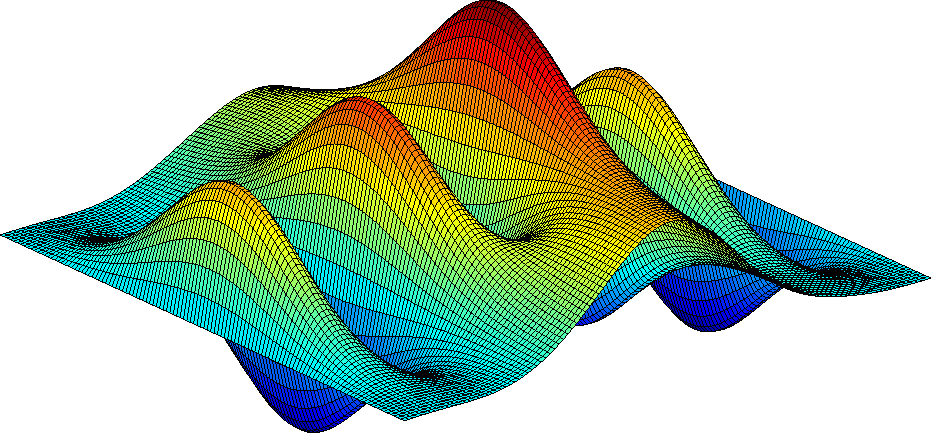
\includegraphics[width=6cm]{plotdata/plotgraphics3dsurf.png}}%
}

现在的关键思路是识别图像中的几个点，并\emph{同时}为它们分配逻辑三维坐标\emph{和}图像坐标中相应的二维画布坐标。如何做？嗯，三维坐标是 Matlab 已知的，如果你点击图像中的某个位置，它可以为你显示这些坐标，比较 Figure~\ref{fig:plotgraphics3d}（左）。


\begin{figure}
    \noindent
    \hbox to \linewidth{\hfill
        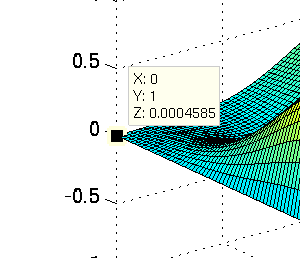
\includegraphics{plotdata/plotgraphics3dsurfmatlab.png}%
        \hfill
        \begin{minipage}[b][4cm][c]{2.6cm}%
        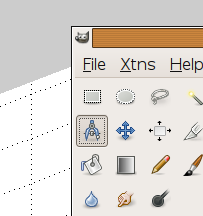
\includegraphics[width=\linewidth]{plotdata/plotgraphics_gimpmeasure.png}%
        \end{minipage}
        \hfill
    }
    \caption{使用 Matlab 提取图像坐标（左）和 Gimp 测量距离（右）。}
        \label{fig:plotgraphics3d}
\end{figure}


二维画布坐标需要一些工作；它们需要相对于图像的\emph{左下角}提供。我使用了 |gimp| 并将单位设为“Points”（左下角）。现在左下角以 |pt| 显示图像坐标，这与 \PGFPlots{} 兼容。指向坐标的替代方法是测量工具；比较 Figure~\ref{fig:plotgraphics3d}（右）中 |gimp| 的“Measure”工具，它允许计算一条线的长度（在我们的情况下，是从左下角到目标点的长度）。

我在图形中选择了四个点，并记录了它们的二维图像坐标和三维逻辑坐标，如下所示：
%
\begin{codeexample}[]
\begin{tikzpicture}
\begin{axis}[
    grid=both,minor tick num=1,
    xlabel=$x$,ylabel=$y$,
]
    \addplot3 graphics [
        points={% important
            (0,1,0) => (0,207-112)
            (1,0,0) => (446,207-133)
            (0.5546,0.5042,1.825) => (236,207)
            (0,0,0) => (194,207-202)
        },
    ] {plotdata/plotgraphics3dsurf.png};
\end{axis}
\end{tikzpicture}
\end{codeexample}
%
这里，|points| 键以我们收集的坐标作为参数。它接受形式为 \meta{3d 逻辑坐标} | => | \meta{2d 画布坐标} 的映射序列。在我们的例子中，|(0,1,0)| 在 |.png| 文件中的 |(0,207-112)| 处被找到。请注意，我引入了差值，因为 |gimp| 从左上角计数，但 \PGFPlots{} 从左下角计数。

一旦收集了这四个点坐标，我们就在 \PGFPlots{} 坐标轴中得到 Matlab 的曲面图。你可以修改任何外观选项，包括不同的坐标轴 limits 或更多 |\addplot| 命令：
%
\begin{codeexample}[]
\begin{tikzpicture}
\begin{axis}[
    xmax=1.5,% extra limits
    grid=both,minor tick num=1,
    xlabel=$x$,ylabel=$y$,
]
    \addplot3 [surf] % 'surf': only used for legend
        graphics [
            points={
                (0,1,0) => (0,207-112)
                (1,0,0) => (446,207-133)
                (0.5546,0.5042,1.825) => (236,207)
                (0,0,0) => (194,207-202)
        },
    ] {plotdata/plotgraphics3dsurf.png};
        \addlegendentry{Graphics}

    \addplot3+ [only marks] coordinates {
        (0,1,0) (1,0,0)
        (0.5546,0.5042,1.825) (0,0,0)
    };
        \addlegendentry{Scatter}
\end{axis}
\end{tikzpicture}
\end{codeexample}
%
\noindent \PGFPlots{} 使用这四个输入点来计算适当的 |x|、|y| 和 |z| 单位向量（以及图形坐标中的原点）。这四个向量（每个有两个分量）可以作为一个大小为 $8\times 8$ 的线性方程组的结果来计算，这就是为什么你需要提供四个输入点（每个有两个坐标）。\PGFPlots{} 计算导入图形的单位向量，然后重新缩放结果，使其适合指定的 |width| 和 |height|。这种重新缩放尊重 |unit vector ratio|（更准确地说，它使用 |scale mode=scale uniformly| 而不是 |scale mode=stretch to fill|）。因此，更改包含投影图形的三维坐标轴视图的自由度比之前小得多。令人惊讶的是，你仍然可以更改坐标轴 limits 以及 |width| 和 |height|——\PGFPlots{} 会负责正确显示你导入的图形。从版本~1.6 开始，你还可以更改 |zmin| 和/或 |zmax|——\PGFPlots{} 会尽可能尊重你的更改。

下面是另一个例子。假设我们有以下三维可视化图形：

{\setlength{\fboxsep}{0pt}%
\centering%
\fbox{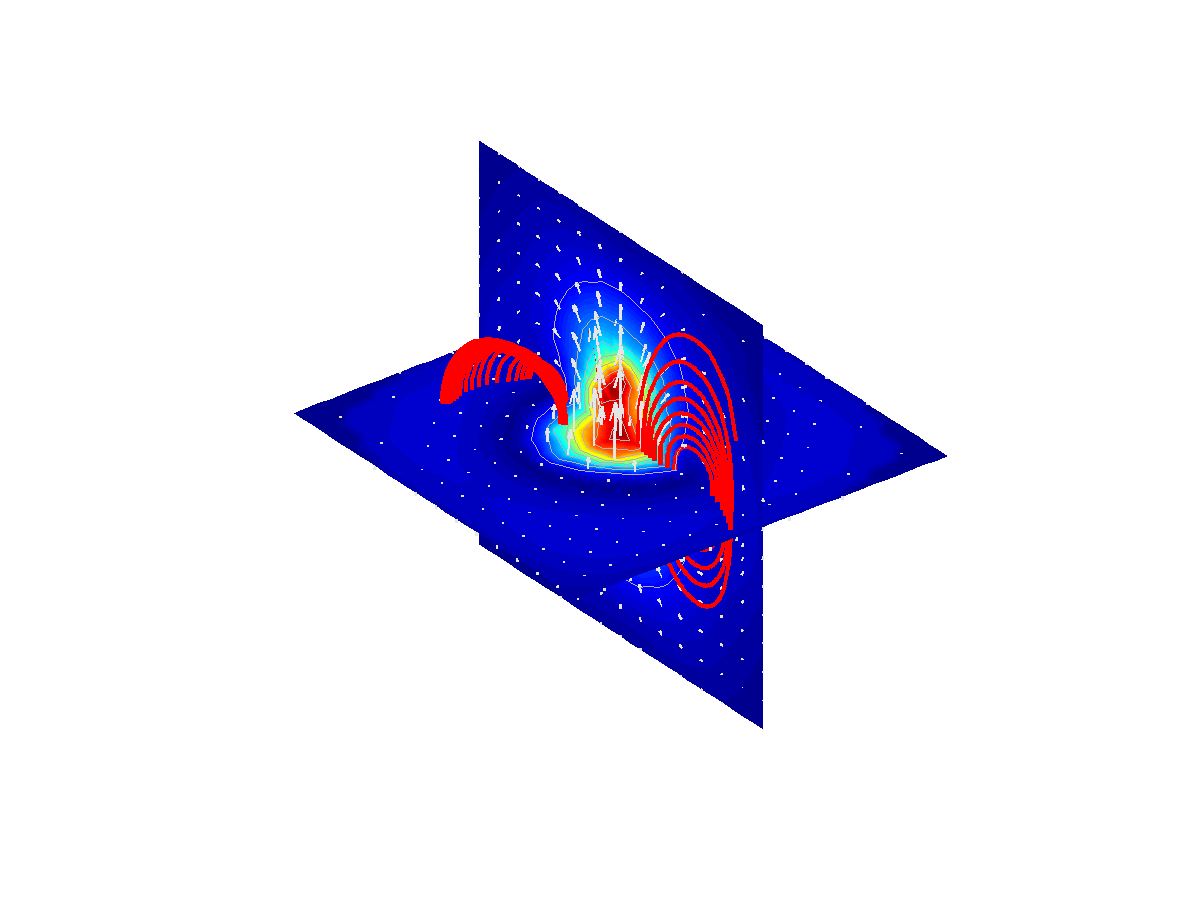
\includegraphics[width=6cm]{plotdata/risingdrop3d}}%
}

它由 Matlab 生成（我只用 |gimp| 为背景添加了透明度）。除了高级可视化技术之外，它还使用了 |axis equal|，即 |unit vector ratio=1 1 1|。和之前一样，我们需要识别四个点，每个点都有其三维逻辑坐标（来自 Matlab）以及相对于图形左下角的相关二维画布坐标（请注意图形周围有大量空白）。以下是导入结果图形时 \PGFPlots{} 的输出：
%
\begin{codeexample}[]
\begin{tikzpicture}
\begin{axis}[
    grid=both,minor tick num=1,
    xlabel=$x$,ylabel=$y$,
    title={\centering
      Geometry provided by Sven Gro\ss, Bonn\\
      \url{http://www.igpm.rwth-aachen.de/DROPS}\\},
    title style={text width=6cm,font=\tiny},
]
    \addplot3 graphics [
        points={
            (-0.002625,0.002625,0) => (140,234)
            (0,0.00263,0.00263)    => (230,364)
            (0,-0.00263,-0.00263)  => (366,81)
            (0,-0.00263,0.00263)   => (366,276)
            (0.002625,0.002625,0.002625)
        },
    ] {plotdata/risingdrop3d.png};
\end{axis}
\end{tikzpicture}
\end{codeexample}
%
\noindent 请注意，我在这里提供了\emph{五个}三维坐标，但最后一项没有 |=>| 映射到二维画布坐标。因此，它仅用于更新边界框（详见 |points| 键的参考手册）。

上面的例子产生了一个相对较小的图像和大量“空白”。这是由于 \PGFPlots{} 的 |scale mode=scale uniformly| 实现：它决定最好的方法是放大相关的坐标轴 limits。这里，“最好的方法”意味着满足 |width|/|height| 约束，同时最小化地放大（从不缩小）坐标轴 limits。剩余的自由度是 |width|、|height| 和坐标轴 limits。在我们的例子中，更改 |width| 和 |height| 之间的比例可以改善显示：

\begin{codeexample}[]
\begin{tikzpicture}
\begin{axis}[
    height=8cm,width=7cm,% improve scaling manually
    grid=both,minor tick num=1,
    xlabel=$x$,ylabel=$y$,
    title={\centering
      Geometry provided by Sven Gro\ss, Bonn\\
      \url{http://www.igpm.rwth-aachen.de/DROPS}\\},
    title style={text width=6cm,font=\tiny},
]
    \addplot3 graphics [
        points={
            (-0.002625,0.002625,0) => (140,234)
            (0,0.00263,0.00263)    => (230,364)
            (0,-0.00263,-0.00263)  => (366,81)
            (0,-0.00263,0.00263)   => (366,276)
            (0.002625,0.002625,0.002625)
        },
    ] {plotdata/risingdrop3d.png};
\end{axis}
\end{tikzpicture}
\end{codeexample}
%
\noindent 发生的事情是，\PGFPlots{} 选择了一个\emph{单一}缩放因子，该因子应用于从 |points| 键推导出来的所有单位。这确保导入的图形正确地适合坐标轴。此外，\PGFPlots{} 会尽力满足剩余的约束。

关于 \PGFPlots{} 如何缩放坐标轴的完整描述可以在 |scale mode=scale uniformly| 的文档中找到。这里只是简要总结：\PGFPlots{} 假设规定的 |width| 和 |height| 必须被满足。为此，它重新缩放投影的单位向量（即 $x$、$y$ 和 $z$ 中每个单位所占用的空间），并且可以修改坐标轴 limits。在默认配置 |scale uniformly strategy=auto| 中，\PGFPlots{} \emph{从不}缩小坐标轴 limits。


\paragraph{兼容性说明：}

请注意，\PGFPlots{} 版本~1.6 的缩放能力已得到改进。在以前的版本中，只有 |scale uniformly strategy=change vertical limits| 可用，这会导致坐标轴被裁剪。简而言之：请考虑在文档中写入 |\pgfplotsset{compat=1.6}| 或更新版本，以受益于改进的缩放。如果你使用 |\pgfplotsset{compat=1.5}| 或更早版本，|\addplot3 graphics| 的结果会有所不同。

我们来看第三个例子，它由以下 Matlab 代码生成：
%
\begin{codeexample}[code only]
clear all
close all
seed = sum(clock)
rand('seed',seed);
X = rand(10,10,10);
data = smooth3(X,'box',5);
p1 = patch(isosurface(data,.5), ...
   'FaceColor','blue','EdgeColor','none');
p2 = patch(isocaps(data,.5), ...
    'FaceColor','interp','EdgeColor','none');
isonormals(data,p1)
daspect([1 2 2])
view(3); axis vis3d tight
camlight; lighting phong
% print -dpng plotgraphics3withaxis
axis off
print -dpng plotgraphics3
save  plotgraphics3.seed seed -ASCII % to reproduce the result
\end{codeexample}
%
\noindent 我只用 |gimp| 添加了背景透明度，得到以下图形：

{\setlength{\fboxsep}{0pt}%
\centering%
\fbox{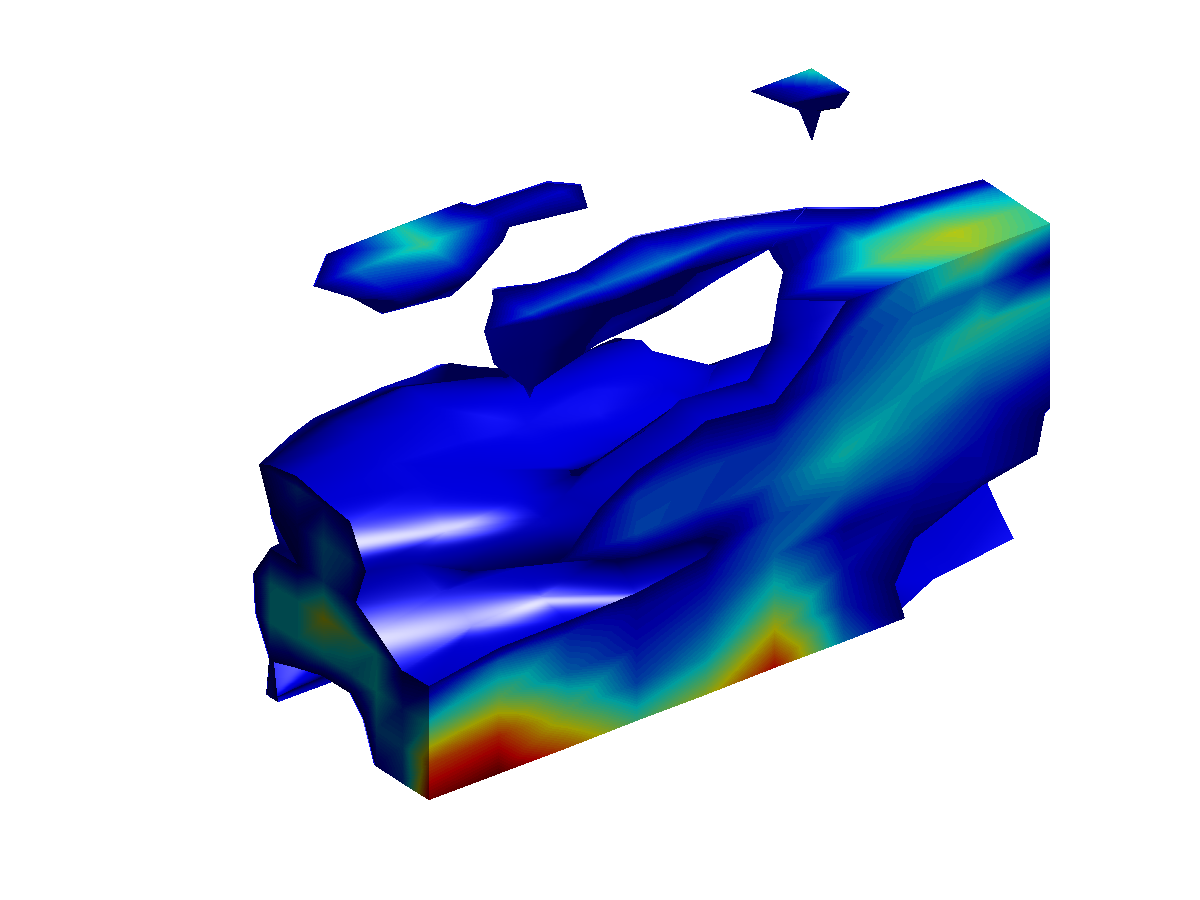
\includegraphics[width=6cm]{plotdata/plotgraphics3.png}}%
}

我们像之前一样继续，收集四个点，每个点都有三维逻辑坐标（通过点击 Matlab 图形）以及使用 gimp 测量工具得到的相关二维画布（图形）坐标。结果如下面的代码示例所示。
%
\begin{codeexample}[]
\begin{tikzpicture}
\begin{axis}[
    grid=both,minor tick num=1,
    xlabel=$x$,ylabel=$y$,
    3d box,
]
    \addplot3 graphics [
        points={
            (1,1,1)    => (205,48)
            (10,1,10)  => (503,324)
            (1,1,4.044)=> (206,102)
            (10,10,10) => (390,398)
        },
    ] {plotdata/plotgraphics3.png};
\end{axis}
\end{tikzpicture}
\end{codeexample}
%
\noindent 请注意，它具有非标准的数据纵横比，\PGFPlots{} 会自动尊重这一点。


\subsection*{外部三维图形与 Matlab}
\label{sec:plotgraphics3d:matlabscript}

\textit{由 Jürnjakob Dugge 提供的扩展} \vskip\baselineskip

\noindent 将三维逻辑坐标映射到二维画布坐标的过程很繁琐。

Jürnjakob Dugge 贡献了一个脚本，它完成了大部分逻辑工作，你的工作简化为复制--粘贴。经他允许，我在此发布该贡献。

其思路是启动一个简单的脚本，它会\emph{记录}用户点击的任何坐标的映射。工作方式如下：
%
\begin{enumerate}
    \item 创建 Matlab 图，例如使用
        %
\begin{codeexample}[code only]
hist3(randn(10000,2)) % some random data
set(get(gca,'child'),'FaceColor','interp','CDataMode','auto'); % colors
% make sure the "print" paper format is the same as the screen paper format:
set(gcf,'PaperPositionMode','auto')
\end{codeexample}
        %
    \item 将以下代码保存为 |pgfplotscsconversion.m|：
        %
\begin{codeexample}[code only]
function pgfplotscsconversion

% Hook into the Data Cursor "click" event
h = datacursormode(gcf);
set(h,'UpdateFcn',@myupdatefcn,'SnapToDataVertex','off');
datacursormode on

% select four points in plot using mouse

% The function that gets called on each Data Cursor click
function [txt] = myupdatefcn(obj,event_obj)

% Get the screen resolution, in dots per inch
dpi = get(0,'ScreenPixelsPerInch');

% Get the click position in pixels, relative to the lower left of the
% screen
screen_location=get(0,'PointerLocation');

% Get the position of the plot window, relative to the lower left of
% the screen
figurePos = get(gcf,'Position');

% Get the data coordinates of the cursor
pos = get(event_obj,'Position');

% Format the data and figure coordinates. The factor "72.27/dpi" is
% necessary to convert from pixels to TeX points (72.27 points per inch)
display(['(',num2str(pos(1)),',',num2str(pos(2)),',',num2str(pos(3)),') => (', ...
   num2str((screen_location(1)-figurePos(1))*72.27/dpi),',', ...
   num2str((screen_location(2)-figurePos(2))*72.27/dpi),')'])

% Format the tooltip display
txt = {['X: ',num2str(pos(1))],['Y: ',num2str(pos(2))],['Z: ',num2str(pos(3))]};
\end{codeexample}
        %
        运行 |pgfplotscsconversion|，在你的图上点击四个点。最好选择靠近图边缘的非共线点。复制并粘贴写入 Matlab 命令窗口的四行内容。

        确保前两个点在屏幕上具有不同的 $X$ 和 $Y$ 值（即图像画布坐标）。
    \item 将图导出为图像
        %
\begin{codeexample}[code only]
axis off
print -dpng matlabout -r400 % PNG called "matlabout.png" with 400 dpi resolution
\end{codeexample}

        如果你想导出矢量图形，应该注意 Matlab 的 |pdf| 输出比较笨拙。最好先导出为 |eps|，然后再从 |eps| 转换为 |pdf|。

        \emph{如果}你真的想使用 Matlab 的 |pdf| 输出，可能需要自己设置纸张大小以匹配图形大小，因为 PDF 驱动程序不会自动调整大小：
        %
\begin{codeexample}[code only]
% It might be better to use print -depsc followed by epstopdf.
% Use this if you (really) want to use print -dpdf:
currentScreenUnits=get(gcf,'Units')     % Get current screen units
currentPaperUnits=get(gcf,'PaperUnits') % Get current paper units
set(gcf,'Units',currentPaperUnits)      % Set screen units to paper units
plotPosition=get(gcf,'Position')        % Get the figure position and size
set(gcf,'PaperSize',plotPosition(3:4))  % Set the paper size to the figure size
set(gcf,'Units',currentScreenUnits)     % Restore the screen units

print -dpdf matlabout      % PDF called "matlabout.pdf"
\end{codeexample}
        %
    \item 将图像包含到你的 \PGFPlots{} 坐标轴中。如果你在图的角上选择了点，你的 |xmin|、|xmax|、|ymin| 和 |ymax| 应该会被自动设置，否则你可能需要自己提供这些值。此外，调整 |width| 和 |height| 可能有助于获得正确的图垂直位置。考虑更改 |zmin| 和/或 |zmax| 以满足你的需求（最好只更改其中一个；否则 \PGFPlots{} 可能无法固定 |height|）。
\end{enumerate}

此贡献来自

\noindent
\url{http://tex.stackexchange.com/questions/52987/3-dimensional-histogram-in-pgfplots} .


\subsection*{总结：外部三维图形}

如前几节所示，\verbpdfref{\addplot3} |graphics| 允许包含三维图形，而 \PGFPlots{} 以其全部能力叠加一个灵活的坐标轴。这样做的代价是：
%
\begin{enumerate}
    \item 为你的图形\emph{四个点}收集逻辑三维坐标\emph{和}图像内部二维坐标。

        在 Matlab 中，可以通过第~\pageref{sec:plotgraphics3d:matlabscript} 页提到的工具来简化。
    \item 如果你的坐标轴构成右手坐标系，那就完成了。如果不是，还要为任何反向的坐标轴添加 |x dir=reverse|。
\end{enumerate}

\noindent 如果你在使用 \verbpdfref{\addplot3} |graphics| 时遇到问题，请考虑以下列表：
%
\begin{itemize}
    \item 必须能够从提供的四个 |points| 推导出原点和三个（二维）单位向量；否则算法将失败。

        算法应该能检测到任何缺陷。不过，如果你在这里遇到奇怪的“Dimension too large”消息，可以尝试 |points| 中的其他参数。查看你的日志文件，它可能会指出问题的根源（或使用 |debug| 键）。
    \item 确保外部图形具有正交坐标轴。事实上，坐标轴可以是倾斜的（就像 \PGFPlots{} 坐标轴可以通过自定义 |x|、|y| 和 |z| 向量创建一样）。不过，外部图像不能有透视投影，因为 \PGFPlots{} 不支持这种。|points| 命令需要接收四个属于线性无关位置向量的点。
    \item \PGFPlots{} 使用前两个点将图形挤压到所需坐标中（这意味着它们不应具有相同的画布 $X$ 或 $Y$ 坐标）。它会验证剩余的 |points| 参数是否被正确投影。
    \item 通过 |scale mode=scale uniformly| 产生的缩放将尝试满足所有缩放约束。你可以通过修改 |width|、|height|、|xmin|、|xmax|、|ymin|、|ymax|、|zmin|、|zmax| 和/或这些参数的任意组合来更改这些约束。另见 |unit rescale keep size|，它控制 limits 更改的灵活性。还有一个键 |scale uniformly strategy|，它允许选择不同的缩放策略。
    \item 图像应该具有“右手坐标系”：你应该能够用右手，拇指指向 $x$ 轴方向，食指指向~$y$ 方向，中指指向 $z$ 轴方向。如果不可能，说明你的某个坐标轴是反向的，你需要通过 |x dir=reverse| 键（及其变体）显式告知 \PGFPlots{}。
    \item 请注意，此功能仅在标准笛卡尔坐标轴上经过验证。
    \item 有一个 |debug| 键可用于调查算法在做什么：
        %
        \begin{pgfplotskey}{plot graphics/debug=\mchoice{true,false,visual} (initially false)}
            如果你提供 |\addplot3 graphics[debug,points={...}]|，\PGFPlots{} 将在你的终端和日志文件中提供调试信息。它还会生成额外的文件，其中包含确定的单位向量和用于推导它们的线性方程组（每个 |\addplot3 graphics| 语句生成一个这样的文件，文件名将是图形文件名加上 |.dat|）。

            如果没有 |debug| 键，只有日志文件会包含关于 \PGFPlots{} 在幕后做什么的简要信息。

            选择 \declaretext{true} 会激活日志消息。选择 \declaretext{visual} 会激活日志消息\emph{并}在提供的 |points| 处放置一些实心圆。选择 \declaretext{false} 会禁用所有 |debug| 功能。
        \end{pgfplotskey}
\end{itemize}
}


\subsection{从文件读取坐标}

\begin{addplotoperation}[]{file}{\marg{name}}
\labelprefix\label{pgfplots:addplot:file}

    \paragraph{弃用说明：}

    如果你有数据文件，通常应该使用 |\addplot table|。输入类型 |\addplot file| 几乎相同，但功能要弱得多。它仅为向后兼容而保留。

    |\addplot file| 输入机制类似于 \Tikz{} 命令 `|\addplot file|'。它应这样使用：

\begin{codeexample}[code only]
\addplot file {datafile.dat};
\end{codeexample}
    %
    其中 \meta{name} 是一个至少有两列的文本文件，这些列将用作 $x$ 和 $y$ 坐标。以 `|%|' 或 `|#|' 开头的行会被忽略。此类文件通常由 \textsc{gnuplot} 生成：
    %
\begin{codeexample}[code only]
#Curve 0, 20 points
#x y type
0.00000 0.00000 i
0.52632 0.50235 i
1.05263 0.86873 i
1.57895 0.99997 i
...
9.47368 -0.04889 i
10.00000 -0.54402 i
\end{codeexample}
    %
    此列表复制自~\cite[Section~16.4]{tikz}。

    Plot file 接受一个可选参数，

\begin{codeexample}[code only]
\addplot file [skip first] {datafile.dat};
\end{codeexample}

    \noindent 它允许跳过一个非注释标题行。这允许通过跳过列名来读取与 |\addplot table| 相同的输入文件。请注意，注释行在这里不计为行。

    输入方法 |\addplot file| 还可以为每个坐标读取元数据。如 |\addplot coordinates| 中已经解释的（见上文），元数据可以用于单独更改每个标记的颜色或其他样式参数。现在，如果 |point meta| 设置为 |explicit| 或 |explicit symbolic|，并且输入方法是 |\addplot file|，则将从磁盘读取一个额外元素——对每一行。元数据始终是读取的最后一个元素。关于逐点元数据的信息和示例见第~\pageref{pgfplots:scatter:src} 页，使用 |scatter/classes| 的应用示例见第~\pageref{pgfplots:scatterclasses} 页。

    Plot file 与 |\addplot table| 非常相似：你可以用以下方式达到相同的效果：
    %
\begin{codeexample}[code only]
\addplot table [x index=0,y index=1,header=false] {datafile.dat};
\end{codeexample}
    %
    \noindent 由于其简单性，|\addplot file| 稍快一些，而 |\addplot table| 允许更高的灵活性。

    技术说明：每个打开的文件都会被记录到你的日志文件中。

    文件可以包含 |empty line|，以告诉 \PGFPlots{} 函数有跳跃。要使用它，只需插入一个空行（并确保你的导言区中有 |\pgfplotsset{compat=1.4}| 或更新版本）。详见 |empty line| 的文档。
\end{addplotoperation}

\begin{pgfplotskeylist}{%
    plot file/skip first=\mchoice{true,false} (initially false),
    plot file/ignore first=\mchoice{true,false} (initially false)%
}
    这两个键可以作为 |\addplot file[|\meta{options}|] |\marg{filename}|;| 的参数提供，以跳过文件中第一个非注释条目。它们是等价的。如果你在此上下文中提供它们，则可以省略前缀 |/pgfplots/plot file|。
\end{pgfplotskeylist}
